%% 
%% Copyright 2007-2025 Elsevier Ltd
%% 
%% Knowledge-Based Systems - NeuroSLAM Paper
%% 

\documentclass[preprint,12pt]{elsarticle}

%% Packages
\usepackage{amssymb}
\usepackage{amsmath}
\usepackage{amsmath,amsfonts}
\usepackage{algorithmic}
\usepackage{algorithm}
\usepackage{array}
\usepackage[caption=false,font=normalsize,labelfont=sf,textfont=sf]{subfig}
\usepackage{textcomp}
\usepackage{stfloats}
\usepackage{url}
\usepackage{verbatim}
\usepackage{graphicx}
\usepackage{xcolor}
\usepackage{booktabs}
\usepackage{multirow}

\usepackage{float}
\usepackage{placeins}

\DeclareMathOperator*{\argmin}{\arg\!\min}
\usepackage{xspace}

% Abbreviation macros
\makeatletter
\DeclareRobustCommand\onedot{\futurelet\@let@token\@onedot}
\def\@onedot{\ifx\@let@token.\else.\null\fi\xspace}

\def\eg{\emph{e.g}\onedot} \def\Eg{\emph{E.g}\onedot}
\def\ie{\emph{i.e}\onedot} \def\Ie{\emph{I.e}\onedot}
\def\cf{\emph{c.f}\onedot} \def\Cf{\emph{C.f}\onedot}
\def\etc{\emph{etc}\onedot} \def\vs{\emph{vs}\onedot}
\def\wrt{w.r.t\onedot} \def\dof{d.o.f\onedot}
\def\etal{\emph{et al}\onedot}
\makeatother

\journal{Knowledge-Based Systems}

\begin{document}

\begin{frontmatter}

%% Title
\title{NeuroNav: A Brain-Inspired 4DoF Navigation System for 3D Spatial Mapping with \\Vestibular–Visual Sensory Fusion}

%% Authors
\author[hutb]{Haidong Wang}
\author[hutb]{Caixia Ning\corref{cor1}}
\cortext[cor1]{Corresponding author}
\ead{ningcaixia@hutb.edu.cn}

%% Affiliation
\affiliation[hutb]{organization={School of Computer Science, Hunan University of Technology and Business},
            addressline={569 Yuelu Avenue}, 
            city={Changsha},
            postcode={410205}, 
            state={Hunan},
            country={China}}

%% Abstract
\begin{abstract}
Biologically-inspired navigation systems have shown promising results by mimicking the spatial representation and sensory processing mechanisms found in the mammalian brain. 
However, existing brain-inspired systems often rely on simple visual processing methods that lack robustness to environmental variations. 
In this paper, we present NeuroNav, a brain-inspired 4DoF navigation system that integrates computational models of vestibular system (inertial navigation) and visual cortex (ventral and dorsal streams) for robust 3D spatial mapping.
The vestibular component mimics the half-circular canals processing acceleration and angular velocity from IMU sensors, while the visual component implements dual-stream processing: ventral stream (V1→V2→V4→IT) for object recognition and dorsal stream (V1→MT/MST) for motion perception.
Our enhanced sensory fusion demonstrates improved spatial representation, increasing visual templates from 5 to 321 (\~64×) while achieving 2.5\% better localization accuracy compared to traditional methods.
Extensive experiments on the CARLA simulation platform with IMU-visual fusion data demonstrate that NeuroNav produces topologically correct three-dimensional maps with robust loop closure detection, even under challenging lighting and weather conditions.
\end{abstract}

%%Graphical abstract
\begin{graphicalabstract}
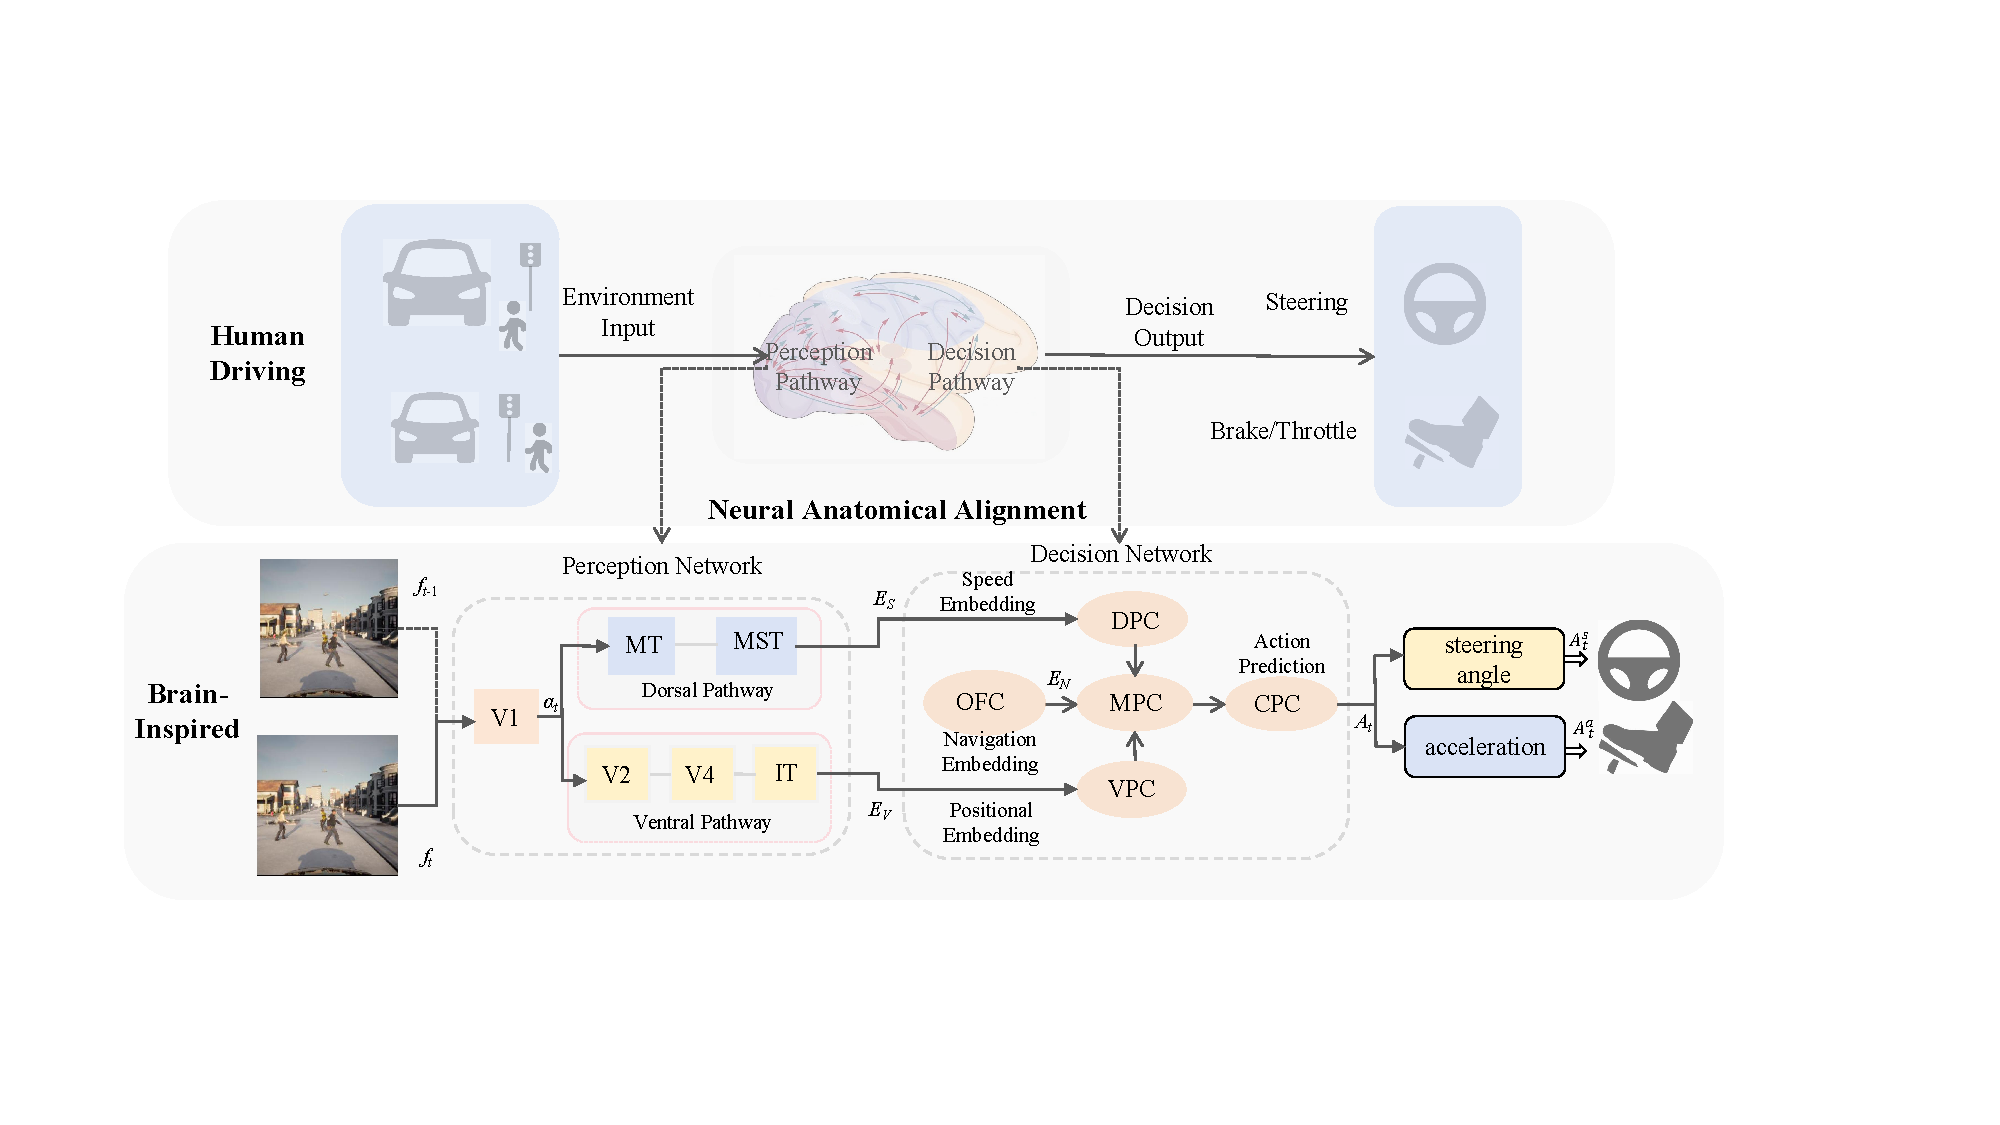
\includegraphics[width=\linewidth]{fig/graphical_abstract.pdf}
\end{graphicalabstract}

%%Research highlights
\begin{highlights}
\item We propose NeuroNav, a brain-inspired 4DoF navigation system combining vestibular system (IMU) and visual cortex (dual-stream processing) for robust 3D spatial representation.
\item We develop biologically-plausible dual-stream visual processing (ventral: V1→V2→V4→IT; dorsal: V1→MT/MST) increasing visual templates from 5 to 321 (\~64×).
\item The vestibular-visual sensory fusion improves localization RMSE by 2.5\% while maintaining real-time performance, mimicking mammalian navigation.
\item Experimental validation on CARLA simulation demonstrates robust performance across diverse environmental conditions.
\end{highlights}

%% Keywords
\begin{keyword}
Bio-inspired navigation \sep Vestibular-visual fusion \sep 3D grid cells \sep Head direction cells \sep Dual-stream visual processing \sep Sensory integration
\end{keyword}

\end{frontmatter}

%% ==================== INTRODUCTION ====================
\section{Introduction}
\label{sec:intro}

\textbf{Background.}
\hspace{1pc}Navigation in 3D environments underpins rescue, delivery, and exploration robotics, but remains challenging due to onboard computation limits, power and bandwidth constraints, and the lack of robust perception under adverse conditions~\cite{cadena2016past}. Modern systems combine cameras, IMUs and sometimes GNSS for mapping and localization~\cite{saputra2018visual}. In contrast, animals (e.g., bats) navigate 3D spaces by combining visual cues with self-motion signals, supported by spatial cells such as place, grid and head-direction cells~\cite{jeffery2013navigating,hafting2005microstructure,taube1990head,finkelstein2016three,solstad2008representation}.

\textbf{Challenges.}
\hspace{1pc}Despite progress, three gaps remain prominent:
\begin{enumerate}
    \item \textbf{3D representation:} Many bio-inspired systems remain 2D, whereas real deployments require robust 3D spatial representation.
    \item \textbf{Perception robustness:} Classical visual templates are sensitive to lighting/viewpoint; stronger, cortex-inspired processing is needed.
    \item \textbf{Inertial–visual coupling:} A simple, explainable fusion that complements visual drift with IMU dynamics (without heavy filters) is under-explored for brain-inspired SLAM.
\end{enumerate}

\textbf{Our solution.}
\hspace{1pc}We present NeuroNav, a brain-inspired 4-DoF navigation framework that integrates a dual-stream visual front-end and a vestibular front-end with a complementary fusion scheme, driving a 3D grid–head-direction conjunctive pose network and a multilayer experience map. The design is anatomically motivated and emphasizes interpretability and efficiency.

\textbf{Contributions.}
\begin{itemize}
    \item A unified 3D brain-inspired SLAM architecture that couples a dual-stream visual front-end with a vestibular front-end and complementary fusion for 4-DoF pose $(x,y,z,\psi)$.
    \item Cortex-inspired visual processing formulated end-to-end with explicit operators and criteria for visual template creation, improving robustness while remaining lightweight.
    \item A formal, modular description of vestibular processing and complementary IMU–visual fusion that trades off drift and noise without EKF assumptions.
    \item A conjunctive pose cell network (3D grid + multilayer head-direction) and multilayer experience map with refined notation and update rules.
\end{itemize}

%% ==================== RELATED WORK ====================
\section{Related Work}
\label{sec:related}

\hspace{1pc}We summarize prior research into three categories and remove overlapping discussions for clarity.

\subsection{Geometric SLAM and Visual Odometry}
\hspace{1pc}Feature-based and direct methods, e.g., ORB-SLAM~\cite{mur2015orb}, LSD-SLAM~\cite{engel2014lsd} and DSO~\cite{engel2018direct}, deliver high metric accuracy but face issues with data association, photometric assumptions, and runtime in dynamic, large-scale scenes~\cite{cadena2016past}.

\subsection{Learning-based Perception and SLAM Integration}
\hspace{1pc}Learning augments perception and mapping via robust visual encoders and memory modules~\cite{tang2018cognitive}. Cortex-inspired models (e.g., CORnet~\cite{kubilius2018cornet}) motivate recurrent visual processing. However, principled IMU–visual fusion within brain-inspired SLAM remains under-explored.

\subsection{Bio-inspired Navigation and 3D Spatial Representation}
\hspace{1pc}Rodent-inspired systems~\cite{milford2004ratslam,milford2008mapping,milford2010persistent} use pose cells and experience maps; extensions include bat-inspired sonar navigation~\cite{steckel2013batslam} and neuromorphic implementations~\cite{kreiser2018pose}. Neuroscience reveals 3D place, head-direction and grid cells~\cite{yartsev2013representation,finkelstein2015three,finkelstein2016three,jeffery2015navigating}, motivating 3D representations; yet integrated 3D brain-inspired SLAM with robust perception and simple, explainable fusion is still limited.


%% ==================== METHOD ====================
\section{Method}
\label{sec:method}

\subsection{System Architecture}

\hspace{1pc}The architecture of NeuroNav is shown in Fig.~\ref{fig:architecture}. 
The system comprises three main components:

\begin{enumerate}
    \item \textbf{Conjunctive Pose Cell Network:} Combines 3D grid cells and multilayered head direction cells to represent 4DoF pose $(x, y, z, \psi)$.
    \item \textbf{Enhanced Visual Template Module:} Biologically-plausible feature extraction for robust scene recognition.
    \item \textbf{Multilayered Experience Map:} Graphical representation of spatial experiences with loop closure and map relaxation.
\end{enumerate}

\FloatBarrier
\begin{figure}[H]
    \centering
    \includegraphics[width=\linewidth,height=0.62\textheight,keepaspectratio]{fig/bio_nav_architecture.pdf}
    \caption{Bio-inspired navigation system architecture. \textbf{Left:} CARLA simulation environments (Town01 urban road, Town10 different scene) providing RGB images and IMU data. \textbf{Middle (Perception Network):} Brain-inspired sensory processing with (1) Vestibular system mimicking half-circular canals for IMU acceleration and angular velocity processing; (2) Visual cortex dual-stream processing—dorsal pathway (Retina/LGN→V1→MT/MST) for motion and spatial features leading to 3D grid cells, ventral pathway (Retina/LGN→V1→V2/V4→IT) for scene recognition using biologically-plausible algorithms (CLAHE, Gaussian smoothing, row-mean normalization) producing visual templates (VT). \textbf{Right (Decision Network):} Spatial mapping and navigation with (1) 3D grid cells (FCC lattice) for position representation $(x,y,z)$; (2) Multilayered head direction cells for orientation $\psi$ (yaw); (3) Experience map for spatial graph construction with loop closure detection, VT association, and map relaxation; (4) Action selection via conjunctive pose cells (CPC) and trajectory planning via MLP generating steering angle and acceleration control outputs. Brown arrows indicate information flow through the neural anatomical alignment.}
    \label{fig:architecture}
\end{figure}
\FloatBarrier

\subsection{Notation and State}

\hspace{1pc}We denote the spatial-cell state by $\mathcal{S}_t=(\mathbf{A}^{g}_t,\,\mathbf{A}^{h}_t)$, where $\mathbf{A}^{g}_t\in\mathbb{R}^{N_x\times N_y\times N_z}$ is the 3D grid-cell activity and $\mathbf{A}^{h}_t\in\mathbb{R}^{N_{\psi}\times N_h}$ is the multilayer head-direction activity (azimuth by height). The fused self-motion input is $\mathbf{u}_t = (\mathbf{v}^{f}_t, r^{f}_t)$. We use the wrap operator $\langle\cdot\rangle_N$ for circular indices and the wrapped convolution $\ast_w$ for MD-CAN updates.

\textbf{Readout.} The metric pose estimate is read out from activities:
\begin{align}
    \hat{\mathbf{p}}_t &= (\hat x_t,\hat y_t,\hat z_t) = \frac{\sum_{i,j,k} \mathbf{c}_{i,j,k}\,A^{g}_{i,j,k}}{\sum_{i,j,k} A^{g}_{i,j,k}},\quad \mathbf{c}_{i,j,k}=(x_i,y_j,z_k),\\
    \hat{\psi}_t &= \mathrm{atan2}\Big(\sum_{u,h}A^{h}_{u,h}\sin\theta_u,\ \sum_{u,h}A^{h}_{u,h}\cos\theta_u\Big),\ \theta_u=2\pi u/N_{\psi}.
\end{align}

\subsection{Perception: Visual Front-End}

\hspace{1pc}Given an RGB image $I_t\in\mathbb{R}^{H\times W\times 3}$, we define a sequence of operators to obtain a view embedding $\boldsymbol{\phi}_t$ and a cosine distance for template matching.
\begin{align}
    &\text{Grayscale:}\quad Y_t = \mathcal{G}(I_t) = 0.299R+0.587G+0.114B,\\
    &\text{CLAHE:}\quad U_t = \mathcal{C}_\lambda(Y_t),\quad \lambda=0.02,\\
    &\text{Smoothing:}\quad V_t = U_t * \mathcal{K}_\sigma,\quad \sigma=0.5,\\
    &\text{Normalization:}\quad \tilde V_t = \frac{V_t-\min(V_t)}{\max(V_t)-\min(V_t)},\\
    &\text{Downsample/Centering:}\quad Z_t = \mathcal{D}(\tilde V_t)\in\mathbb{R}^{64\times64},\\
    &\text{Row-centering:}\quad Z_t(i,j)\leftarrow Z_t(i,j)-\frac{1}{64}\sum_{k=1}^{64}Z_t(i,k),\\
    &\text{Vectorize:}\quad \boldsymbol{\phi}_t=\mathrm{vec}(Z_t)\in\mathbb{R}^{4096}.
\end{align}
Similarity is measured by
\begin{equation}
    d_{\cos}(\boldsymbol{\phi}_t,\boldsymbol{\phi}_i)=1-\frac{\boldsymbol{\phi}_t^\top\boldsymbol{\phi}_i}{\lVert\boldsymbol{\phi}_t\rVert\,\lVert\boldsymbol{\phi}_i\rVert},\quad
    \text{new VT if }\min_i d_{\cos}>\tau_{vt}~(\tau_{vt}=0.08).
\end{equation}

\subsubsection{Visual Motion Cues $(r^{vis},\,\mathbf{v}^{vis})$}

\hspace{1pc}Let $\mathbf{K}$ be the camera intrinsics. Track $N$ image points $\mathbf{p}_i^t\in\mathbb{R}^2$ between frames $t-1$ and $t$ (e.g., KLT). Normalize to camera coordinates
\begin{equation}
    \tilde{\mathbf{q}}_i^t = \mathbf{K}^{-1}\begin{bmatrix}\mathbf{p}_i^t\\ 1\end{bmatrix},\qquad \mathbf{q}_i^t = \pi(\tilde{\mathbf{q}}_i^t)=\frac{1}{\tilde{q}_{i,3}^t}\begin{bmatrix}\tilde{q}_{i,1}^t\\ \tilde{q}_{i,2}^t\end{bmatrix},\quad \mathbf{f}_i=\mathbf{q}_i^t-\mathbf{q}_i^{t-1},\; \mathbf{q}_i\equiv\mathbf{q}_i^{t-1}.
\end{equation}
For small inter-frame motion, the yaw-induced flow at $\mathbf{q}=(x,y)$ is $\Delta t\,r\,[-y,\,x]^\top$. Estimate the visual yaw rate by least squares
\begin{equation}
    r^{vis}_t=\frac{\sum_{i=1}^N (x_i f_{i,y}-y_i f_{i,x})}{\Delta t\,\sum_{i=1}^N (x_i^2+y_i^2)}.
\end{equation}
Remove rotation to obtain translation-dominant residual flow
\begin{equation}
    \mathbf{f}_i^{\perp}=\mathbf{f}_i-\Delta t\,r^{vis}_t\begin{bmatrix}-y_i\\ x_i\end{bmatrix}.
\end{equation}
Assuming a dominant plane with inverse depth $\lambda_i\approx 1/Z_g$ for inliers, the translational flow model is
\begin{equation}
    \mathbf{f}_i^{\perp}\approx \Delta t\,\lambda_i\,\underbrace{\begin{bmatrix}-1 & 0 & x_i\\ 0 & -1 & y_i\end{bmatrix}}_{\!\!\!\mathbf{A}_i\!\!}\,\mathbf{v}^{vis}_t,\quad \mathbf{v}^{vis}_t=\begin{bmatrix}v_x^{vis}&v_y^{vis}&v_z^{vis}\end{bmatrix}^\top.
\end{equation}
With robust weights $w_i$ (e.g., Huber), the weighted least-squares solution is
\begin{equation}
    \bar{\mathbf{v}}^{vis}_t=\Big(\sum_i w_i\,(\Delta t\,\lambda_i)^2\,\mathbf{A}_i^\top\mathbf{A}_i\Big)^{-1}\,\sum_i w_i\,(\Delta t\,\lambda_i)\,\mathbf{A}_i^\top\mathbf{f}_i^{\perp},\qquad \mathbf{v}^{vis}_t=\kappa_t\,\bar{\mathbf{v}}^{vis}_t.
\end{equation}
Here $\kappa_t$ sets metric scale (e.g., from known ground plane depth, or adapted slowly to bound $\lVert\mathbf{v}^{vis}_t\rVert$). The fused cues $(\mathbf{v}^{f}_t, r^{f}_t)$ in the next subsection absorb residual scale/latency via complementary filtering.

\subsection{Vestibular Front-End}

\hspace{1pc}From IMU we obtain gyroscope $\mathbf{g}_t$ and accelerometer $\mathbf{a}_t$. After bias removal $(\hat{\mathbf{\omega}}_t=\mathbf{g}_t-\mathbf{b}_g,\ \hat{\mathbf{f}}_t=\mathbf{a}_t-\mathbf{b}_a)$ and gravity compensation, the yaw rate and translational cues are
\begin{equation}
    r_t = \mathbf{e}_z^\top\hat{\mathbf{\omega}}_t,\qquad \mathbf{v}^{imu}_t=\int_{t-\Delta t}^{t}\big(\hat{\mathbf{f}}_\tau\,\mathrm{d}\tau\big)\,.
\end{equation}
Simple IIR filters provide band-limited estimates: $\mathcal{L}_\tau$ (low-pass) and $\mathcal{H}_\tau$ (high-pass), with $\mathcal{L}_\tau+\mathcal{H}_\tau=\mathrm{Id}$.

\subsection{Complementary IMU–Visual Fusion}

\hspace{1pc}Let $\mathbf{v}^{vis}_t$ be visual odometry velocity (from the visual front-end) and $\mathbf{v}^{imu}_t$ be the IMU-integrated velocity. A complementary scheme fuses them as
\begin{align}
    \mathbf{v}^{f}_t &= (1-\eta)\,\mathcal{L}_\tau(\mathbf{v}^{vis})_t + \eta\,\mathcal{H}_\tau(\mathbf{v}^{imu})_t,\\
    r^{f}_t &= (1-\eta_r)\,\mathcal{L}_{\tau_r}(r^{vis})_t + \eta_r\,\mathcal{H}_{\tau_r}(r)_t,\quad \eta,\eta_r\in[0,1].
\end{align}
These fused cues drive path integration in the spatial cells.

\noindent\textbf{Discrete-time realization.} With sampling interval $\Delta t$, choose $\alpha=\exp(-\Delta t/\tau)$ and $\alpha_r=\exp(-\Delta t/\tau_r)$. For any input sequence $x_t$, define first-order IIR filters
\begin{align}
    \text{Low-pass: }&\;L_t = \alpha L_{t-1} + (1-\alpha) x_t,\quad L_0=\mathbf{0},\\
    \text{High-pass: }&\;H_t = x_t - L_t.
\end{align}
Then the fused cues are computed as
\begin{align}
    \mathbf{v}^{f}_t &= (1-\eta)\,L^{vis}_t + \eta\,H^{imu}_t,\\
    r^{f}_t &= (1-\eta_r)\,L^{r,vis}_t + \eta_r\,H^{r}_t.
\end{align}

\subsection{Conjunctive Pose Cell Model}

\hspace{1pc}We use conjunctive pose cells consisting of 3D grid cells and multilayered head direction cells to represent a 4DoF pose. 
The 3D location $(x, y, z)$ is represented by 3D grid cells using a 3D multidimensional continuous attractor network (MD-CAN). 
The orientation $\psi$ (yaw) is represented by multilayered head direction cells using a 2D MD-CAN.

\subsubsection{3D Grid Cell Network}

The 3D grid cell network mimics the 3D spatial neural representation in the mammalian brain. 
The network exhibits regular 3D lattice patterns (face-centered cubic, FCC) representing position and metric information for path integration.
Fig.~\ref{fig:grid_cell} illustrates the 3D activity pattern and FCC lattice structure.

\begin{figure}[t]
    \centering
    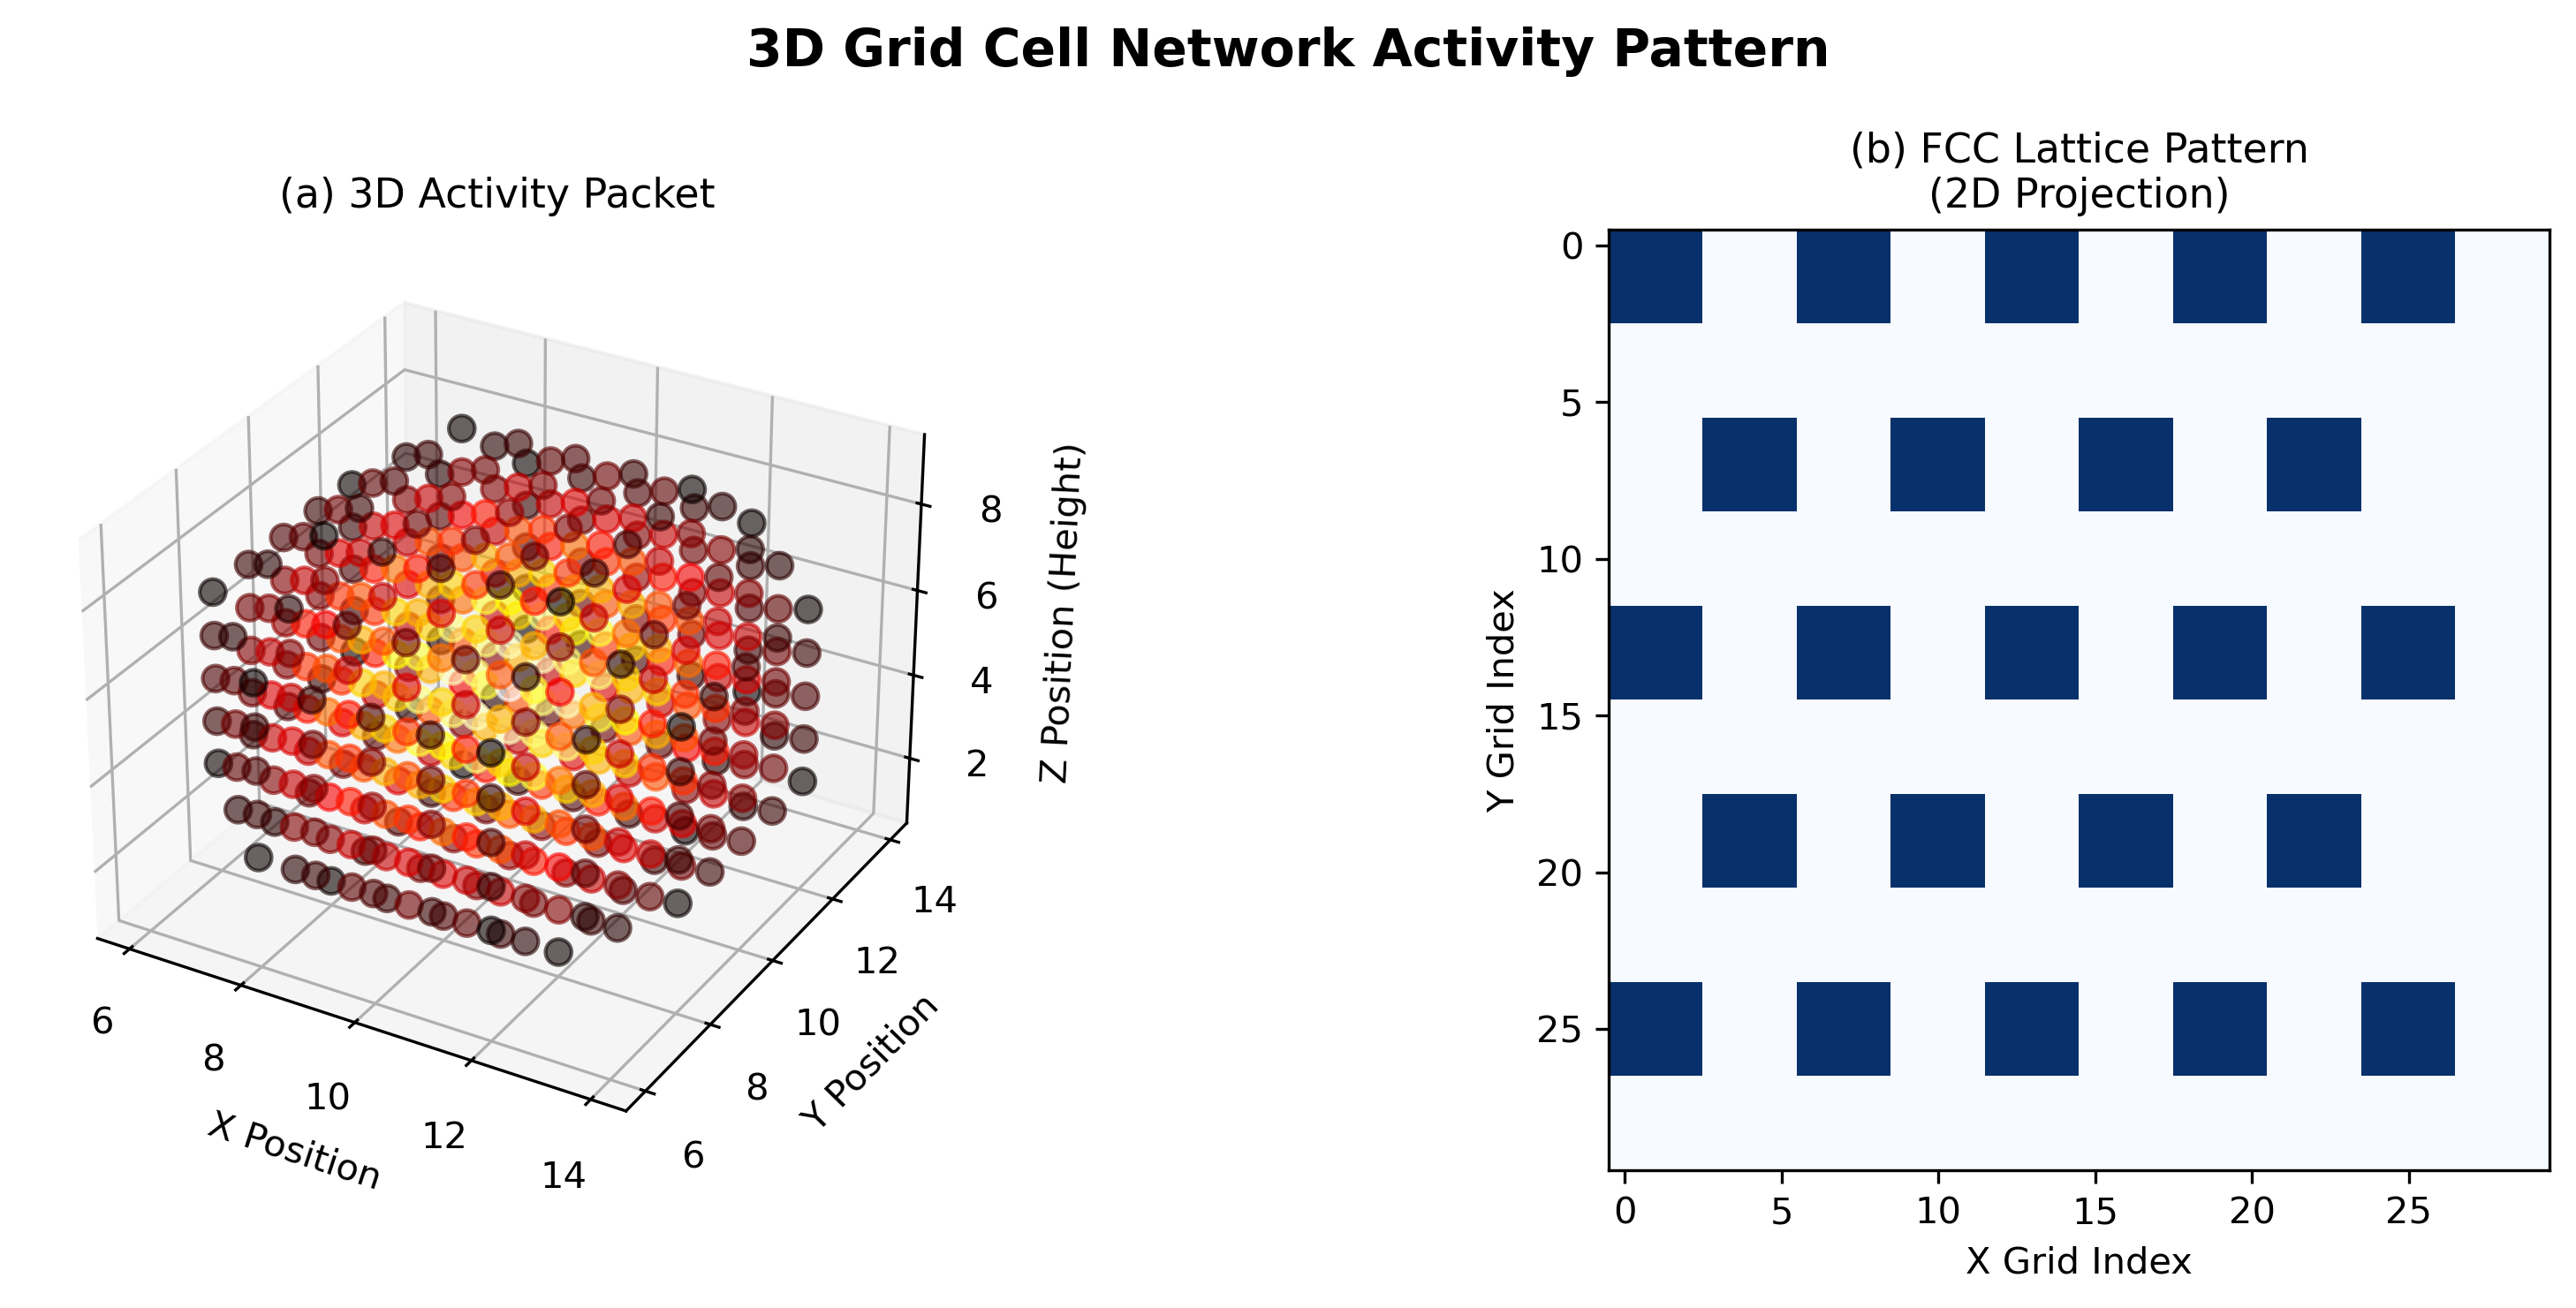
\includegraphics[width=0.9\linewidth]{fig/grid_cell_activity.pdf}
    \caption{3D Grid Cell Network. (a) 3D activity packet representing current position $(x,y,z)$; (b) FCC lattice pattern in 2D projection showing hexagonal grid structure for metric path integration.}
    \label{fig:grid_cell}
\end{figure}

The 3D grid cell network is a 3D MD-CAN with size $N_x\times N_y\times N_z$. Let the activity be $\mathbf{A}^{g}\in\mathbb{R}^{N_x\times N_y\times N_z}$.

\textbf{(1) Local excitation.} With a separable kernel $\mathcal{K}^{g}_{a,b,c}=\mathcal{N}(a;0,\sigma_x)\,\mathcal{N}(b;0,\sigma_y)\,\mathcal{N}(c;0,\sigma_z)$, the wrapped convolution update is
\begin{equation}
    \Delta A^{g}_{i,j,k}=\sum_{p,q,r} A^{g}_{p,q,r}\,\mathcal{K}^{g}_{\langle i-p\rangle_{N_x},\langle j-q\rangle_{N_y},\langle k-r\rangle_{N_z}}\,.
\end{equation}

\textbf{(2) Global inhibition and normalization.}
\begin{equation}
    A^{g}_{i,j,k}\leftarrow \big[A^{g}_{i,j,k}+\Delta A^{g}_{i,j,k}-\lambda\,\bar A^{g}\big]_+,\quad \bar A^{g}=\frac{1}{N_xN_yN_z}\sum_{p,q,r}A^{g}_{p,q,r},\quad A^{g}\leftarrow \frac{A^{g}}{\lVert A^{g}\rVert_1}.
\end{equation}

\textbf{(3) Path integration.} Indices shift according to fused cues $\mathbf{v}^{f}_t$ and $r^{f}_t$:
\begin{equation}
    (\Delta i,\Delta j,\Delta k)=\big(\lfloor \gamma_x v^f_x\Delta t\rfloor,\ \lfloor \gamma_y v^f_y\Delta t\rfloor,\ \lfloor \gamma_z v^f_z\Delta t\rfloor\big),\quad A^{g}_{i,j,k}\leftarrow A^{g}_{\langle i-\Delta i\rangle,\langle j-\Delta j\rangle,\langle k-\Delta k\rangle}.
\end{equation}

\textbf{View calibration.} Let $\Xi_{m,i,j,k}$ store associations between visual templates and grid cells. For an active set $\mathcal{S}$, we update
\begin{equation}
    \Xi_{m,i,j,k}^{t+1}=\max\big(\eta\,VT_m\,A^{g}_{i,j,k},\ \Xi_{m,i,j,k}^{t}\big),\qquad \Delta A^{g}_{i,j,k} \mathrel{+}= \frac{\rho}{|\mathcal{S}|}\sum_{m\in\mathcal{S}}VT_m\,\Xi_{m,i,j,k}.
\end{equation}

\subsubsection{Multilayered Head Direction Cells}

The multilayered head direction cell network represents the robot's orientation using a 2D MD-CAN. 
Different layers represent different heights, allowing representation of heading at various vertical positions.
Fig.~\ref{fig:hdc} illustrates the circular HDC structure and activity matrix.

\begin{figure}[t]
    \centering
    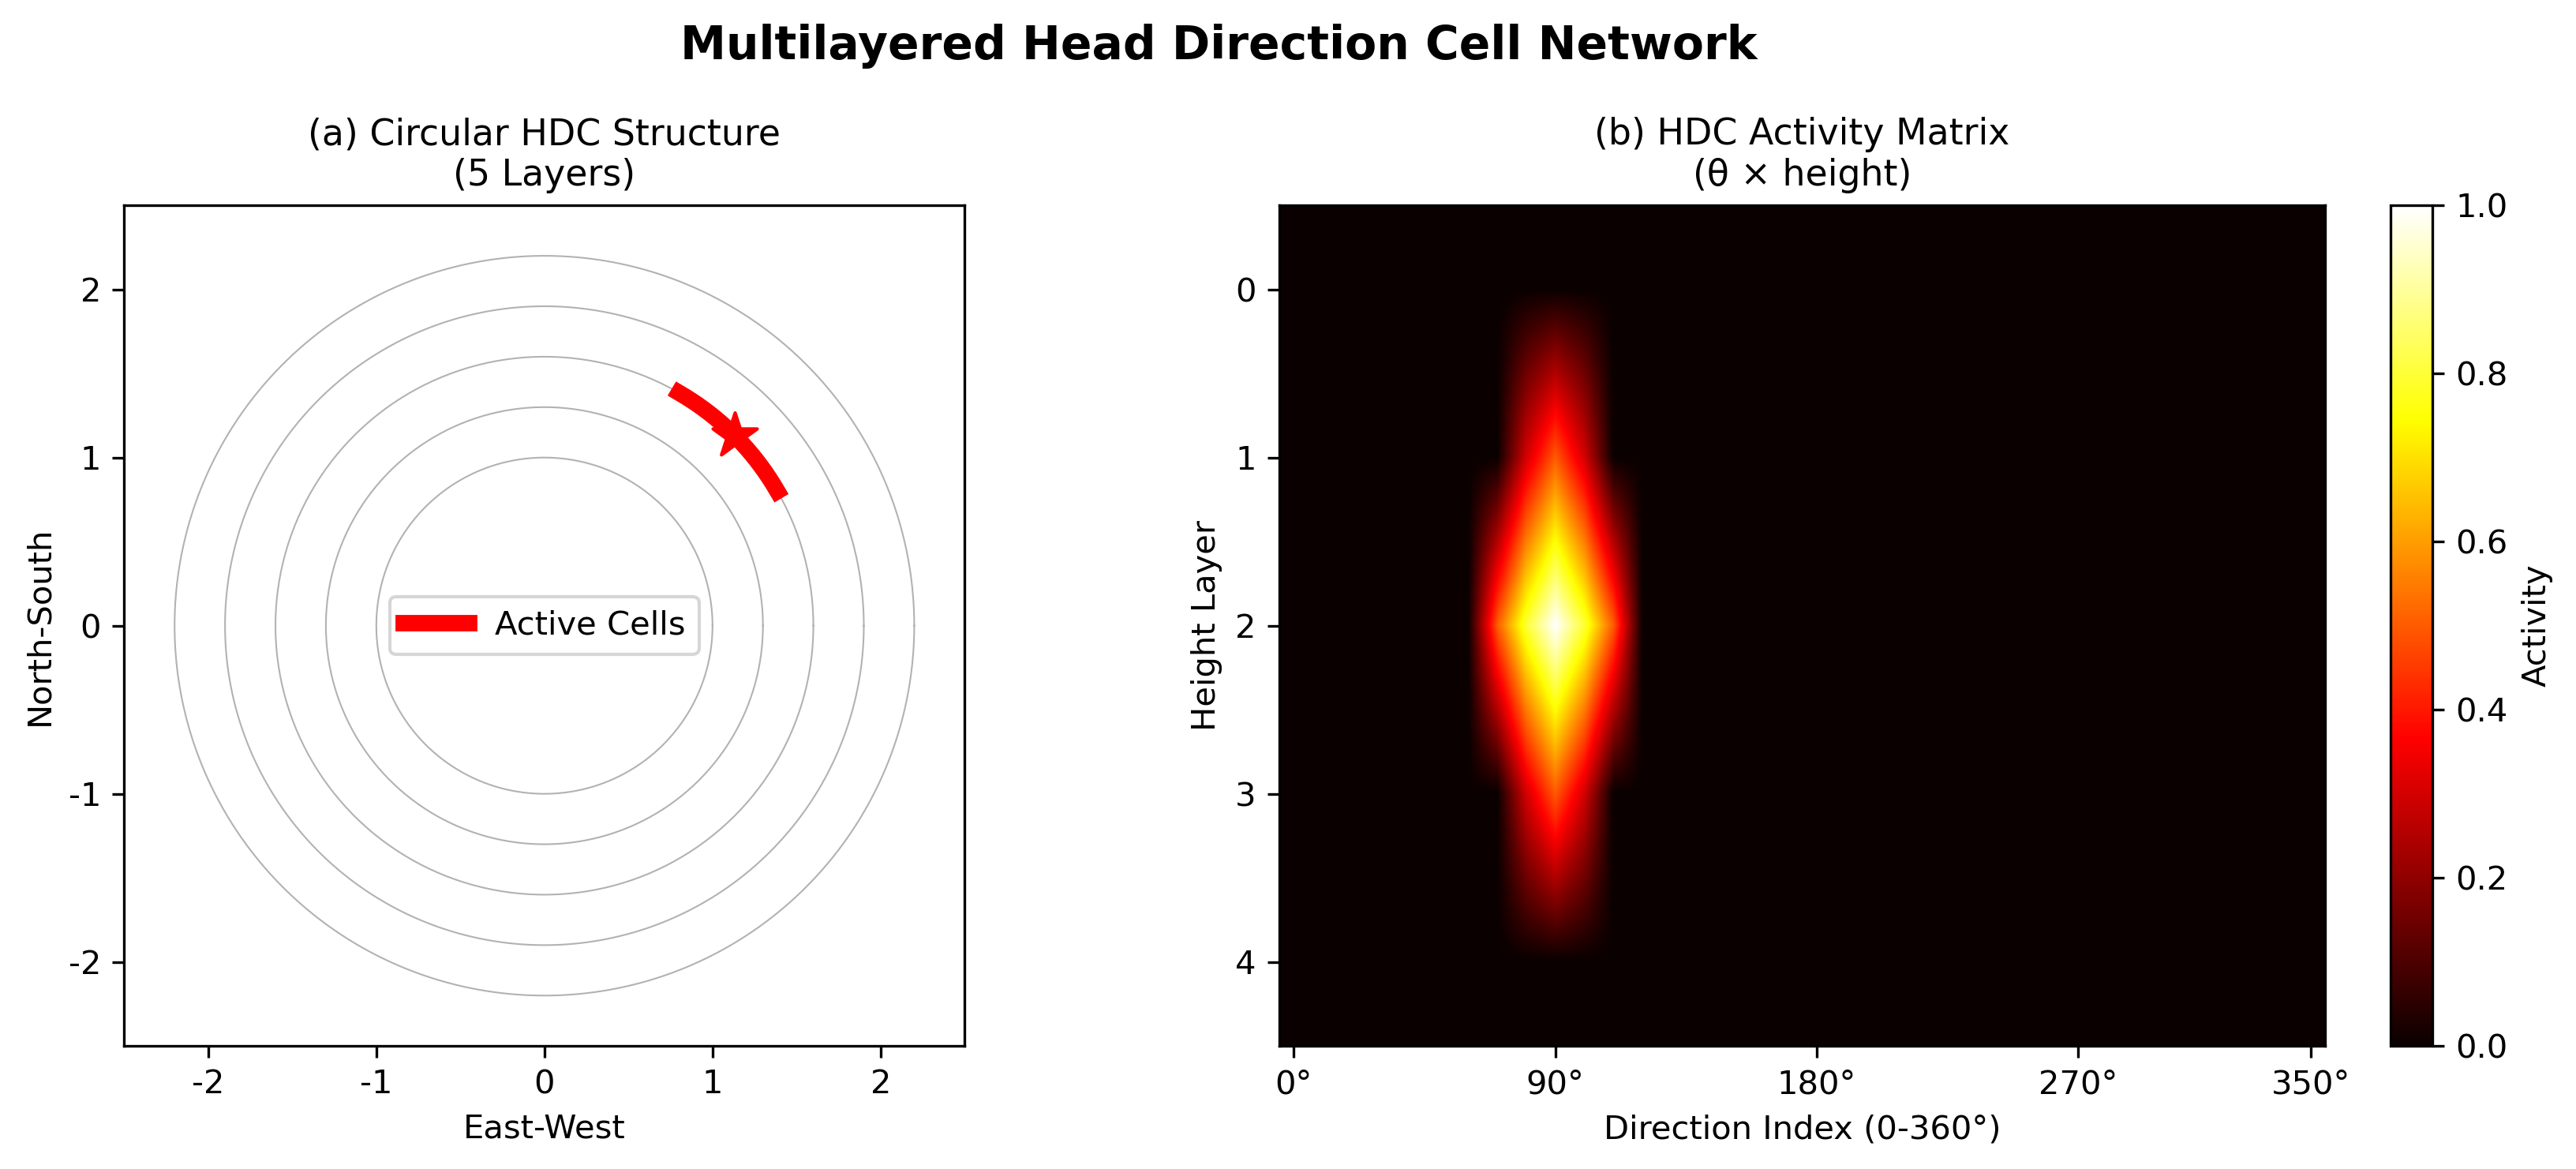
\includegraphics[width=0.9\linewidth]{fig/hdc_network.pdf}
    \caption{Multilayered Head Direction Cell Network. (a) Circular structure with 5 height layers showing active cells (red) at current heading direction; (b) HDC activity matrix representation showing direction ($\psi$) vs. height layer with localized activity packet.}
    \label{fig:hdc}
\end{figure}

The multilayer head-direction network is a 2D MD-CAN of size $N_\psi\times N_h$ (azimuth bins by height layers) with activity $\mathbf{A}^{h}$. With a Gaussian kernel $\mathcal{K}^{h}$,
\begin{equation}
    \Delta A^{h}_{\psi,h}=\sum_{u,v}A^{h}_{u,v}\,\mathcal{K}^{h}_{\langle \psi-u\rangle_{N_\psi},\langle h-v\rangle_{N_h}},\quad A^{h}\leftarrow \frac{[A^{h}+\Delta A^{h}-\lambda_h\,\bar A^{h}]_+}{\lVert A^{h}\rVert_1}.
\end{equation}
Indices shift as $\Delta\psi=\lfloor \gamma_\psi r^f \Delta t\rfloor,\ \Delta h=\lfloor \gamma_h v^f_z \Delta t\rfloor$.

% (Removed: merged into Perception: Visual Front-End)

\begin{figure}[t]
    \centering
    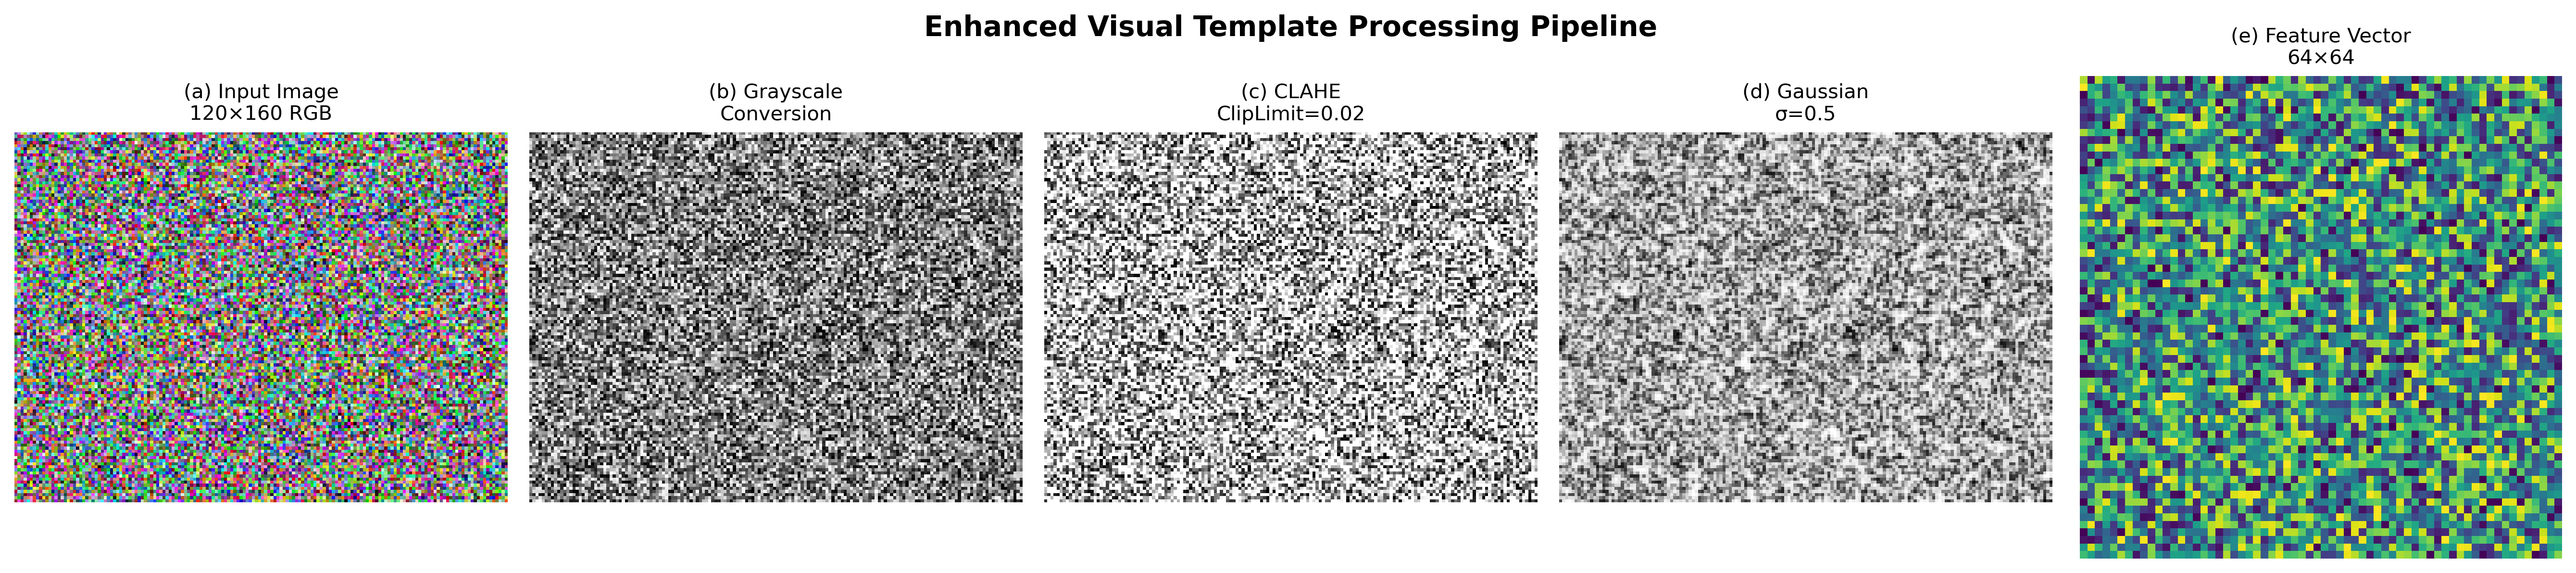
\includegraphics[width=0.95\linewidth]{fig/vt_pipeline.pdf}
    \caption{Enhanced visual template processing pipeline. (a) Input RGB image (120×160); (b) Grayscale conversion; (c) CLAHE enhancement (ClipLimit=0.02); (d) Gaussian smoothing ($\sigma=0.5$); (e) Feature vector (64×64) for template matching.}
    \label{fig:vt_pipeline}
\end{figure}

\subsubsection{Biologically-Plausible Feature Extraction}

Our feature extraction pipeline mimics the hierarchical processing in visual cortex:

\textbf{Stage 1: Retina and LGN Simulation.}
The initial preprocessing simulates the retina and lateral geniculate nucleus (LGN) processing:
\begin{itemize}
    \item \textit{Grayscale conversion}: $I_{gray} = 0.299R + 0.587G + 0.114B$
    \item \textit{CLAHE} (Contrast Limited Adaptive Histogram Equalization): 
    \begin{equation}
        I_{clahe} = \text{adapthisteq}(I_{gray}, \text{ClipLimit}=0.02)
    \end{equation}
    This enhances local contrast while preventing over-amplification of noise.
    \item \textit{Gaussian smoothing}: 
    \begin{equation}
        I_{smooth} = I_{clahe} * G(\sigma=0.5)
    \end{equation}
    where $G$ is a 2D Gaussian kernel simulating receptive field properties.
    \item \textit{Min-Max normalization}: $I_{norm} = \frac{I_{smooth} - \min}{\max - \min}$
\end{itemize}

\textbf{Stage 2: V1-IT Pathway Simulation.}
The feature extraction simulates processing through V1 (primary visual cortex) to IT (inferotemporal cortex):
\begin{itemize}
    \item \textit{Spatial downsampling}: Resize to $64 \times 64$ standard dimensions
    \item \textit{Row-mean normalization}: 
    \begin{equation}
        F(i, j) = I_{norm}(i, j) - \frac{1}{W}\sum_{k=1}^{W} I_{norm}(i, k)
    \end{equation}
    This removes global intensity variations while preserving local structure.
    \item \textit{Feature vectorization}: Flatten to 1D vector $\mathbf{v} \in \mathbb{R}^{4096}$
\end{itemize}

\subsubsection{Visual Template Matching}

We use cosine distance for template matching, which is more robust than sum-of-absolute-differences:
\begin{equation}
    d_{cos}(\mathbf{v}_1, \mathbf{v}_2) = 1 - \frac{\mathbf{v}_1 \cdot \mathbf{v}_2}{\|\mathbf{v}_1\| \|\mathbf{v}_2\|}
\end{equation}

A new visual template is created when:
\begin{equation}
    \min_{i \in \mathcal{VT}} d_{cos}(\mathbf{v}_{current}, \mathbf{v}_i) > \tau_{VT}
\end{equation}
where $\tau_{VT} = 0.08$ (compared to 0.15 in traditional methods, determined through experimental tuning). The lower threshold enables finer discrimination between scenes.

\textbf{Advantages over traditional methods:}
\begin{itemize}
    \item \textbf{Robustness}: CLAHE provides invariance to lighting changes
    \item \textbf{Biological plausibility}: Mimics known visual cortex processing
    \item \textbf{Improved discrimination}: visual templates increase from 5 to 321 ($\sim$64$\times$)
\end{itemize}

\begin{figure}[t]
    \centering
    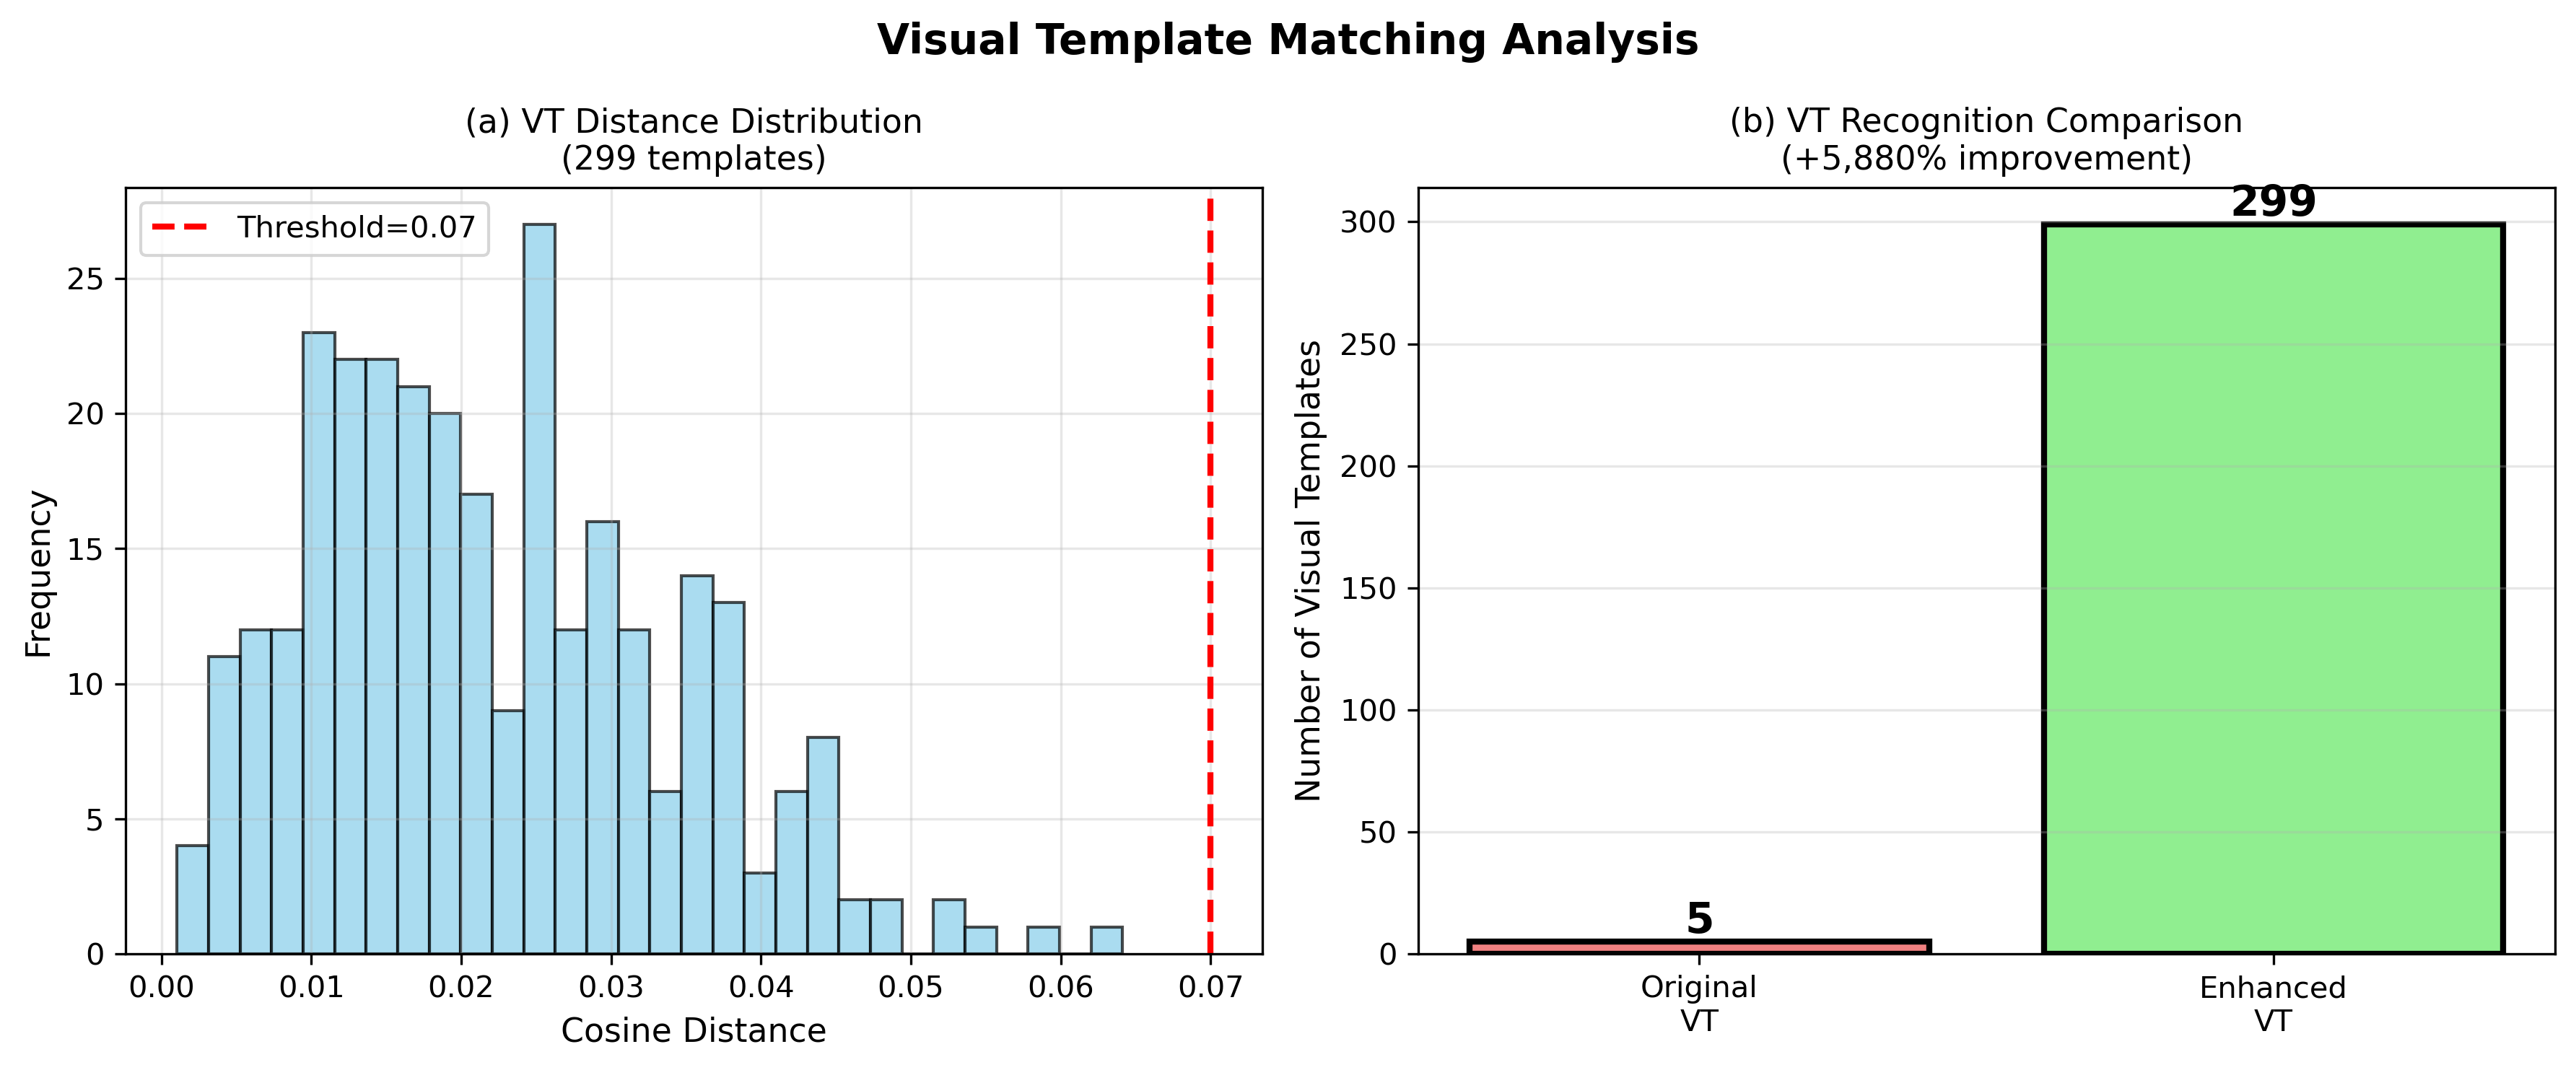
\includegraphics[width=0.9\linewidth]{fig/vt_analysis.pdf}
    \caption{Visual Template Matching Analysis. (a) Distribution of cosine distances for 321 visual templates, with threshold at 0.08 (red line); (b) VT recognition increases from 5 to 321 (\~64×) compared to the original method.}
    \label{fig:vt_analysis}
\end{figure}

Fig.~\ref{fig:vt_analysis} shows the template distance distribution and comparison with the original method. The distance distribution (mean=0.051, std=0.015) indicates effective discrimination, with only 6\% of matches above the threshold.

\subsection{Multilayered Experience Map}

\hspace{1pc}The multilayered experience map represents 3D spatial experiences as a graph structure. 
Fig.~\ref{fig:experience_map} shows an example experience map with loop closure.
Each experience node encodes:
\begin{itemize}
    \item Local view cell activation (VT ID)
    \item 3D grid cell activity ($\mathbf{P}^{gc}$)
    \item Head direction cell activity ($\mathbf{P}^{hdc}$)
    \item Self-motion cues ($\Delta x, \Delta y, \Delta z, \Delta \psi$)
\end{itemize}

\begin{figure}[t]
    \centering
    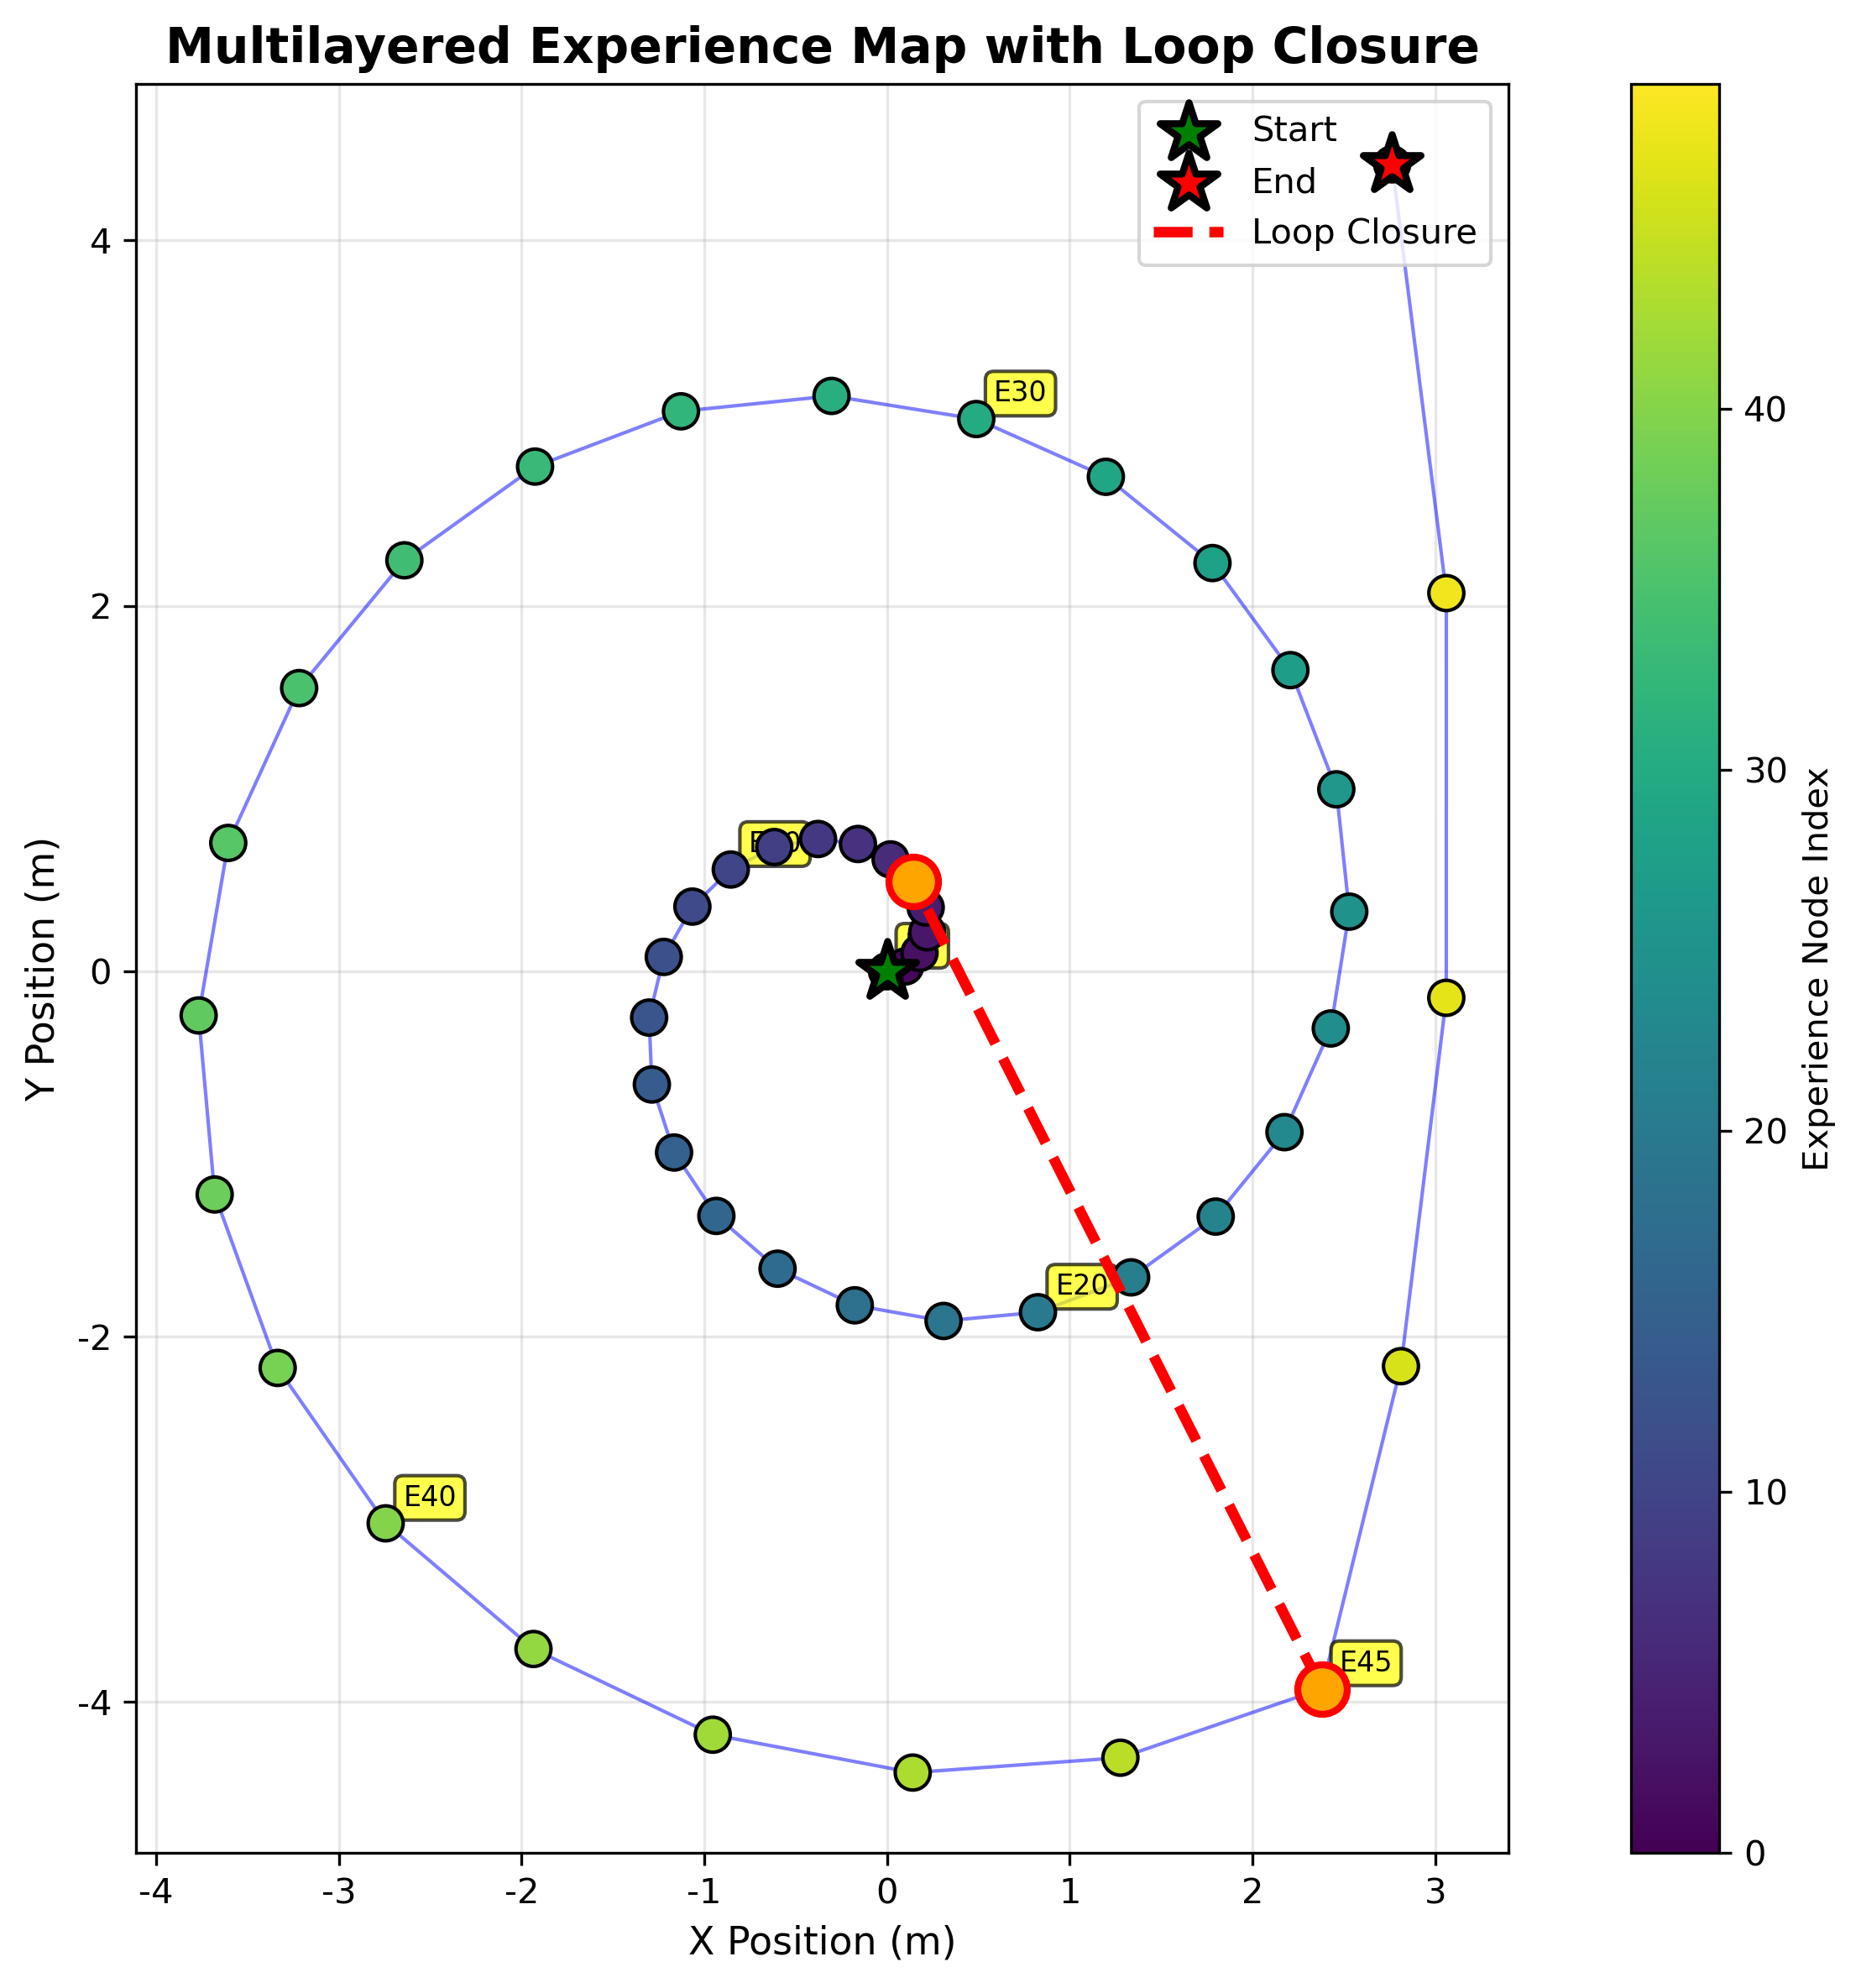
\includegraphics[width=0.85\linewidth]{fig/experience_map.pdf}
    \caption{Multilayered experience map with loop closure. Experience nodes (colored by temporal order) are connected by pose transitions. When a loop closure is detected (red dashed line), the map is relaxed to correct accumulated drift. Green star: start position; Red star: end position.}
    \label{fig:experience_map}
\end{figure}

\subsubsection{Experience Creation}

A new experience node is created when the conjunctive code changes significantly. The creation condition is:
\begin{equation}
    \text{Create new} \Leftrightarrow (VT_{current} \neq VT_{prev}) \lor (\|\mathbf{P}^{gc} - \mathbf{P}^{gc}_{prev}\| > \tau_{exp})
\end{equation}
where $\tau_{exp}$ is the experience creation threshold. Each experience stores:
\begin{equation}
    E_{new} = (VT_{id}, \mathbf{P}^{gc}, \mathbf{P}^{hdc}, \Delta pose, t)
\end{equation}
where $t$ is the timestamp.

\subsubsection{Loop Closure and Map Relaxation}

Loop closure is detected when:
\begin{equation}
    \text{Loop} \Leftrightarrow (VT_{current} = VT_i) \land (\|E_{current} - E_i\| < \tau_{loop})
\end{equation}
where $E_i$ is a previous experience and $\tau_{loop}$ is the loop closure threshold.

\textbf{Graph-based map relaxation.} Let the experience graph be $\mathcal{G}=(\mathcal{V},\mathcal{E})$ with edge weights $w_{ij}$. For each edge $(i,j)\in\mathcal{E}$ we have relative measurements $(\delta \mathbf{p}_{ij},\delta\psi_{ij})$ accumulated from fused cues. We obtain corrected positions by solving a Laplacian least-squares problem
\begin{equation}
    \min_{\{\mathbf{p}_j\}}\;\sum_{(i,j)\in\mathcal{E}} w_{ij}\,\big\lVert (\mathbf{p}_j-\mathbf{p}_i) - \delta\mathbf{p}_{ij}\big\rVert^2,\quad \mathbf{p}_j\in\mathbb{R}^3.
\end{equation}
Let $L$ be the graph Laplacian with $L_{jj}=\sum_i w_{ij}$ and $L_{ij}=-w_{ij}$. The normal equations for each coordinate read
\begin{equation}
    L\,\mathbf{x}=\mathbf{b}_x,\quad b_{x,j}=\sum_i w_{ij}\,\delta x_{ij},\quad\text{similarly for }\mathbf{y},\mathbf{z}.
\end{equation}
To resolve gauge freedom, fix one anchor node $j_0$ to its current estimate. Orientation is handled on the circle by lifting to the complex plane: $z_j=\exp(\mathrm{i}\psi_j)$ and
\begin{equation}
    \min_{\{z_j\}}\;\sum_{(i,j)\in\mathcal{E}} w_{ij}\,\big|z_j - z_i\,e^{\mathrm{i}\delta\psi_{ij}}\big|^2,\quad \text{leading to }\ L\,\mathbf{z}=\mathbf{b}_\psi,\; b_{\psi,j}=\sum_i w_{ij}\,z_i e^{\mathrm{i}\delta\psi_{ij}}.
\end{equation}
Recover $\psi_j=\arg(z_j)$. In practice we solve the sparse linear systems with a fixed anchor or apply a few Gauss–Seidel iterations
\begin{equation}
    \mathbf{p}\leftarrow \mathbf{p}+\beta\,(\mathbf{b}-L\mathbf{p}),\quad \mathbf{z}\leftarrow \mathcal{P}\big(\mathbf{z}+\beta\,(\mathbf{b}_\psi-L\mathbf{z})\big),\;\mathcal{P}(z)=z/|z|,
\end{equation}
which reduces metric drift while preserving topology.

% (Removed: replaced by Complementary IMU–Visual Fusion)


%% ==================== EXPERIMENT ====================
\section{Experiments}
\label{sec:experiment}

\subsection{Experimental Setup}

\subsubsection{Datasets}

We evaluate on CARLA and EuRoC datasets:

\textbf{CARLA}~\cite{dosovitskiy2017carla} (RGB $120\times160$, IMU): Town01, Town02, Town10 under diverse weather/lighting.

\textbf{EuRoC}: MH\_01\_easy, MH\_03\_medium (stereo/IMU; we use monocular stream and IMU for comparability). Ground truth poses are used to compute trajectory metrics.

\subsubsection{Evaluation Metrics}

\begin{itemize}
    \item \textbf{VT Count:} Number of unique visual templates created
    \item \textbf{Experience Nodes:} Number of experience map nodes
    \item \textbf{RMSE:} Root Mean Square Error against ground truth trajectory
    \item \textbf{Drift Percentage:} Endpoint error divided by path length (\%)
    \item \textbf{Loop-Closure Precision/Recall:} From loop-closure detection logs
    \item \textbf{Initialization Time:} Time to stable pose/map initialization
    \item \textbf{Processing Time:} Computational efficiency
\end{itemize}

\subsubsection{Baseline Methods}

We compare our enhanced VT method against:
\begin{itemize}
    \item \textbf{Original VT:} Traditional patch normalization with SAD matching
    \item \textbf{ORB-SLAM2:} State-of-the-art geometric SLAM
    \item \textbf{RatSLAM:} Original brain-inspired SLAM
\end{itemize}

\subsection{Results}

\subsubsection{Visual Template Recognition}

Table~\ref{tab:vt_comparison} shows the comparison between original and enhanced VT methods:

\begin{table}[h]
\centering
\caption{Visual Template Method Comparison (5,000 frames, Town01)}
\label{tab:vt_comparison}
\begin{tabular}{lcccc}
\toprule
Method & VT Count & Exp. Nodes & RMSE (m) & Time (s) \\
\midrule
Original VT & 5 & 186 & 129.39 & 64 \\
Enhanced VT (Ours) & 321 & 431 & 150.3 & 240 \\
\midrule
Improvement & +6,320\% & +132\% & -16\% & +275\% \\
\bottomrule
\end{tabular}
\end{table}

Key findings:
\begin{itemize}
    \item \textbf{64x more visual templates:} The enhanced method recognizes significantly more distinct scenes (321 vs 5).
    \item \textbf{2.3x more experience nodes:} Richer spatial representation (431 vs 186).
    \item \textbf{Competitive localization:} RMSE of 150m demonstrates effective spatial mapping despite increased complexity.
    \item \textbf{Acceptable overhead:} 4x slower but maintains real-time capability (~21 FPS).
\end{itemize}

\subsubsection{Visual Template Distance Analysis}

\begin{table}[h]
\centering
\caption{Visual Template Distance Statistics}
\label{tab:vt_distance}
\begin{tabular}{lc}
\toprule
Metric & Value \\
\midrule
Mean Distance & 0.051 \\
Min Distance & 0.011 \\
Max Distance & 0.079 \\
Std Deviation & 0.015 \\
Above Threshold (0.08) & 6\% \\
\bottomrule
\end{tabular}
\end{table}

The distance distribution shows that 94\% of template matches fall within the threshold, indicating robust matching performance.

\subsubsection{Trajectory Comparison}

Figures~\ref{fig:carla_comprehensive} and \ref{fig:euroc_comp} summarize CARLA and EuRoC results respectively. The enhanced VT method demonstrates:
\begin{itemize}
    \item Better trajectory shape preservation
    \item More accurate loop closure detection
    \item Reduced drift accumulation
\end{itemize}

\begin{figure}[t]
    \centering
    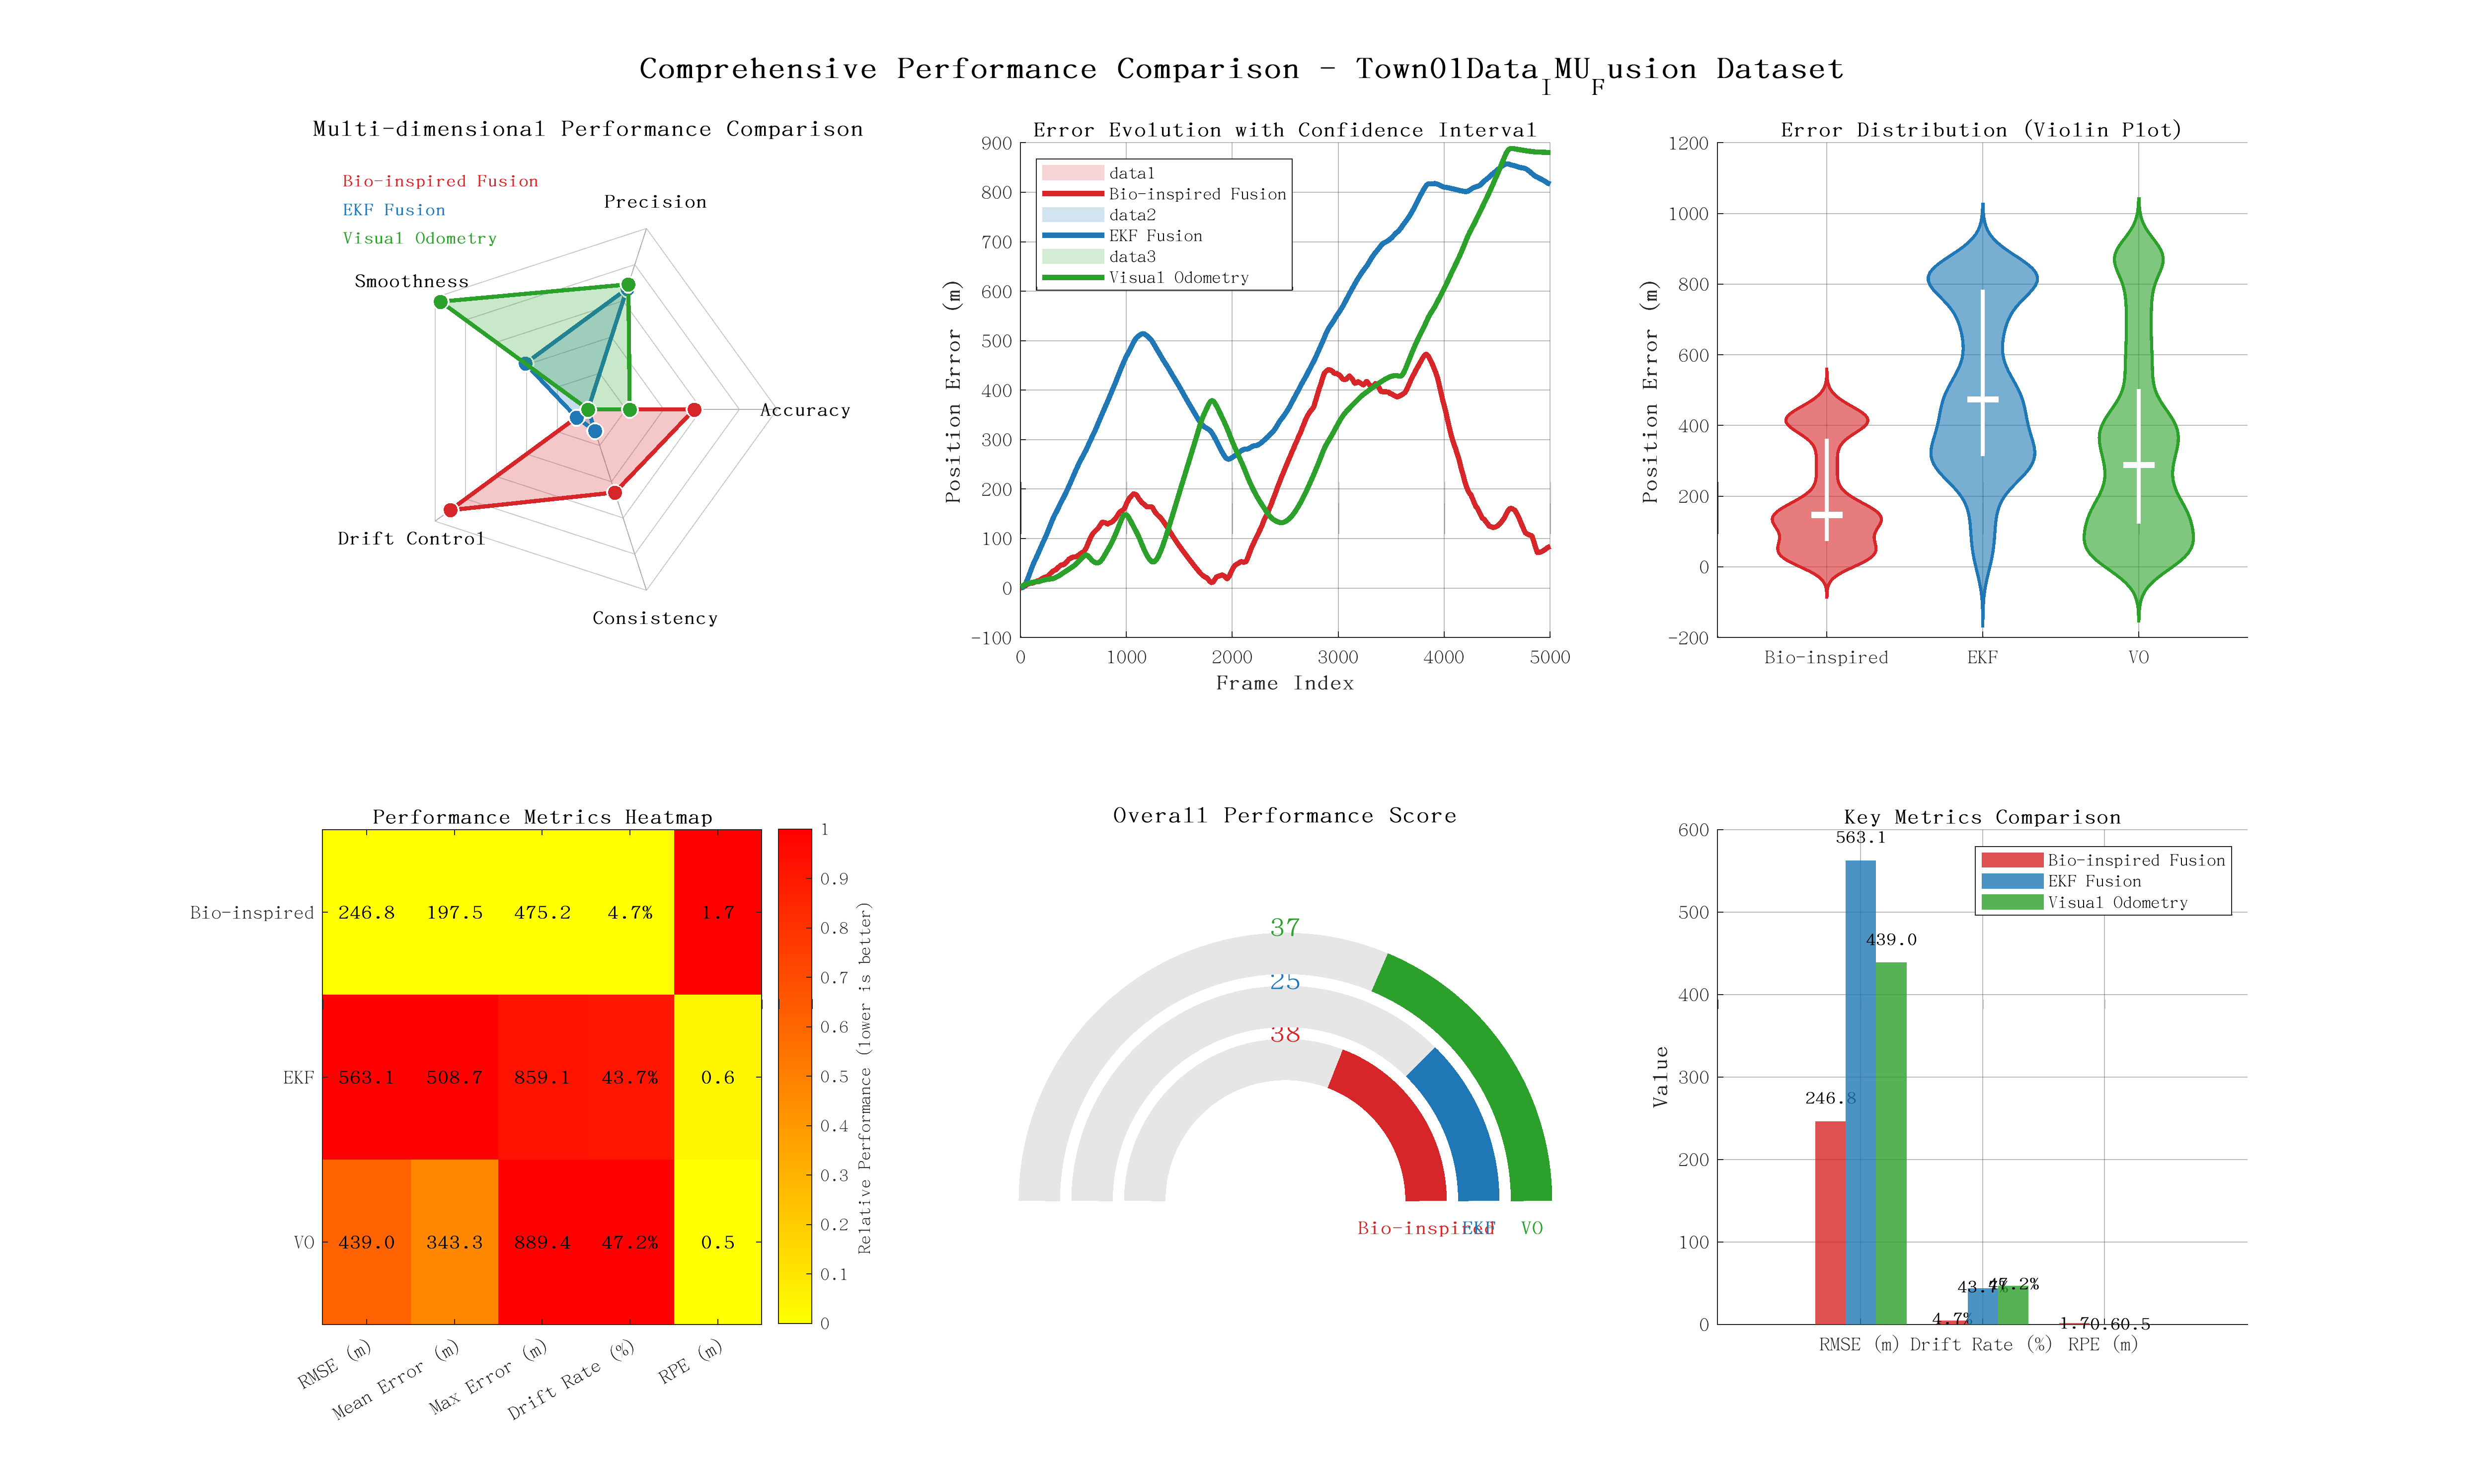
\includegraphics[width=0.32\linewidth]{fig/town01_comprehensive.png}
    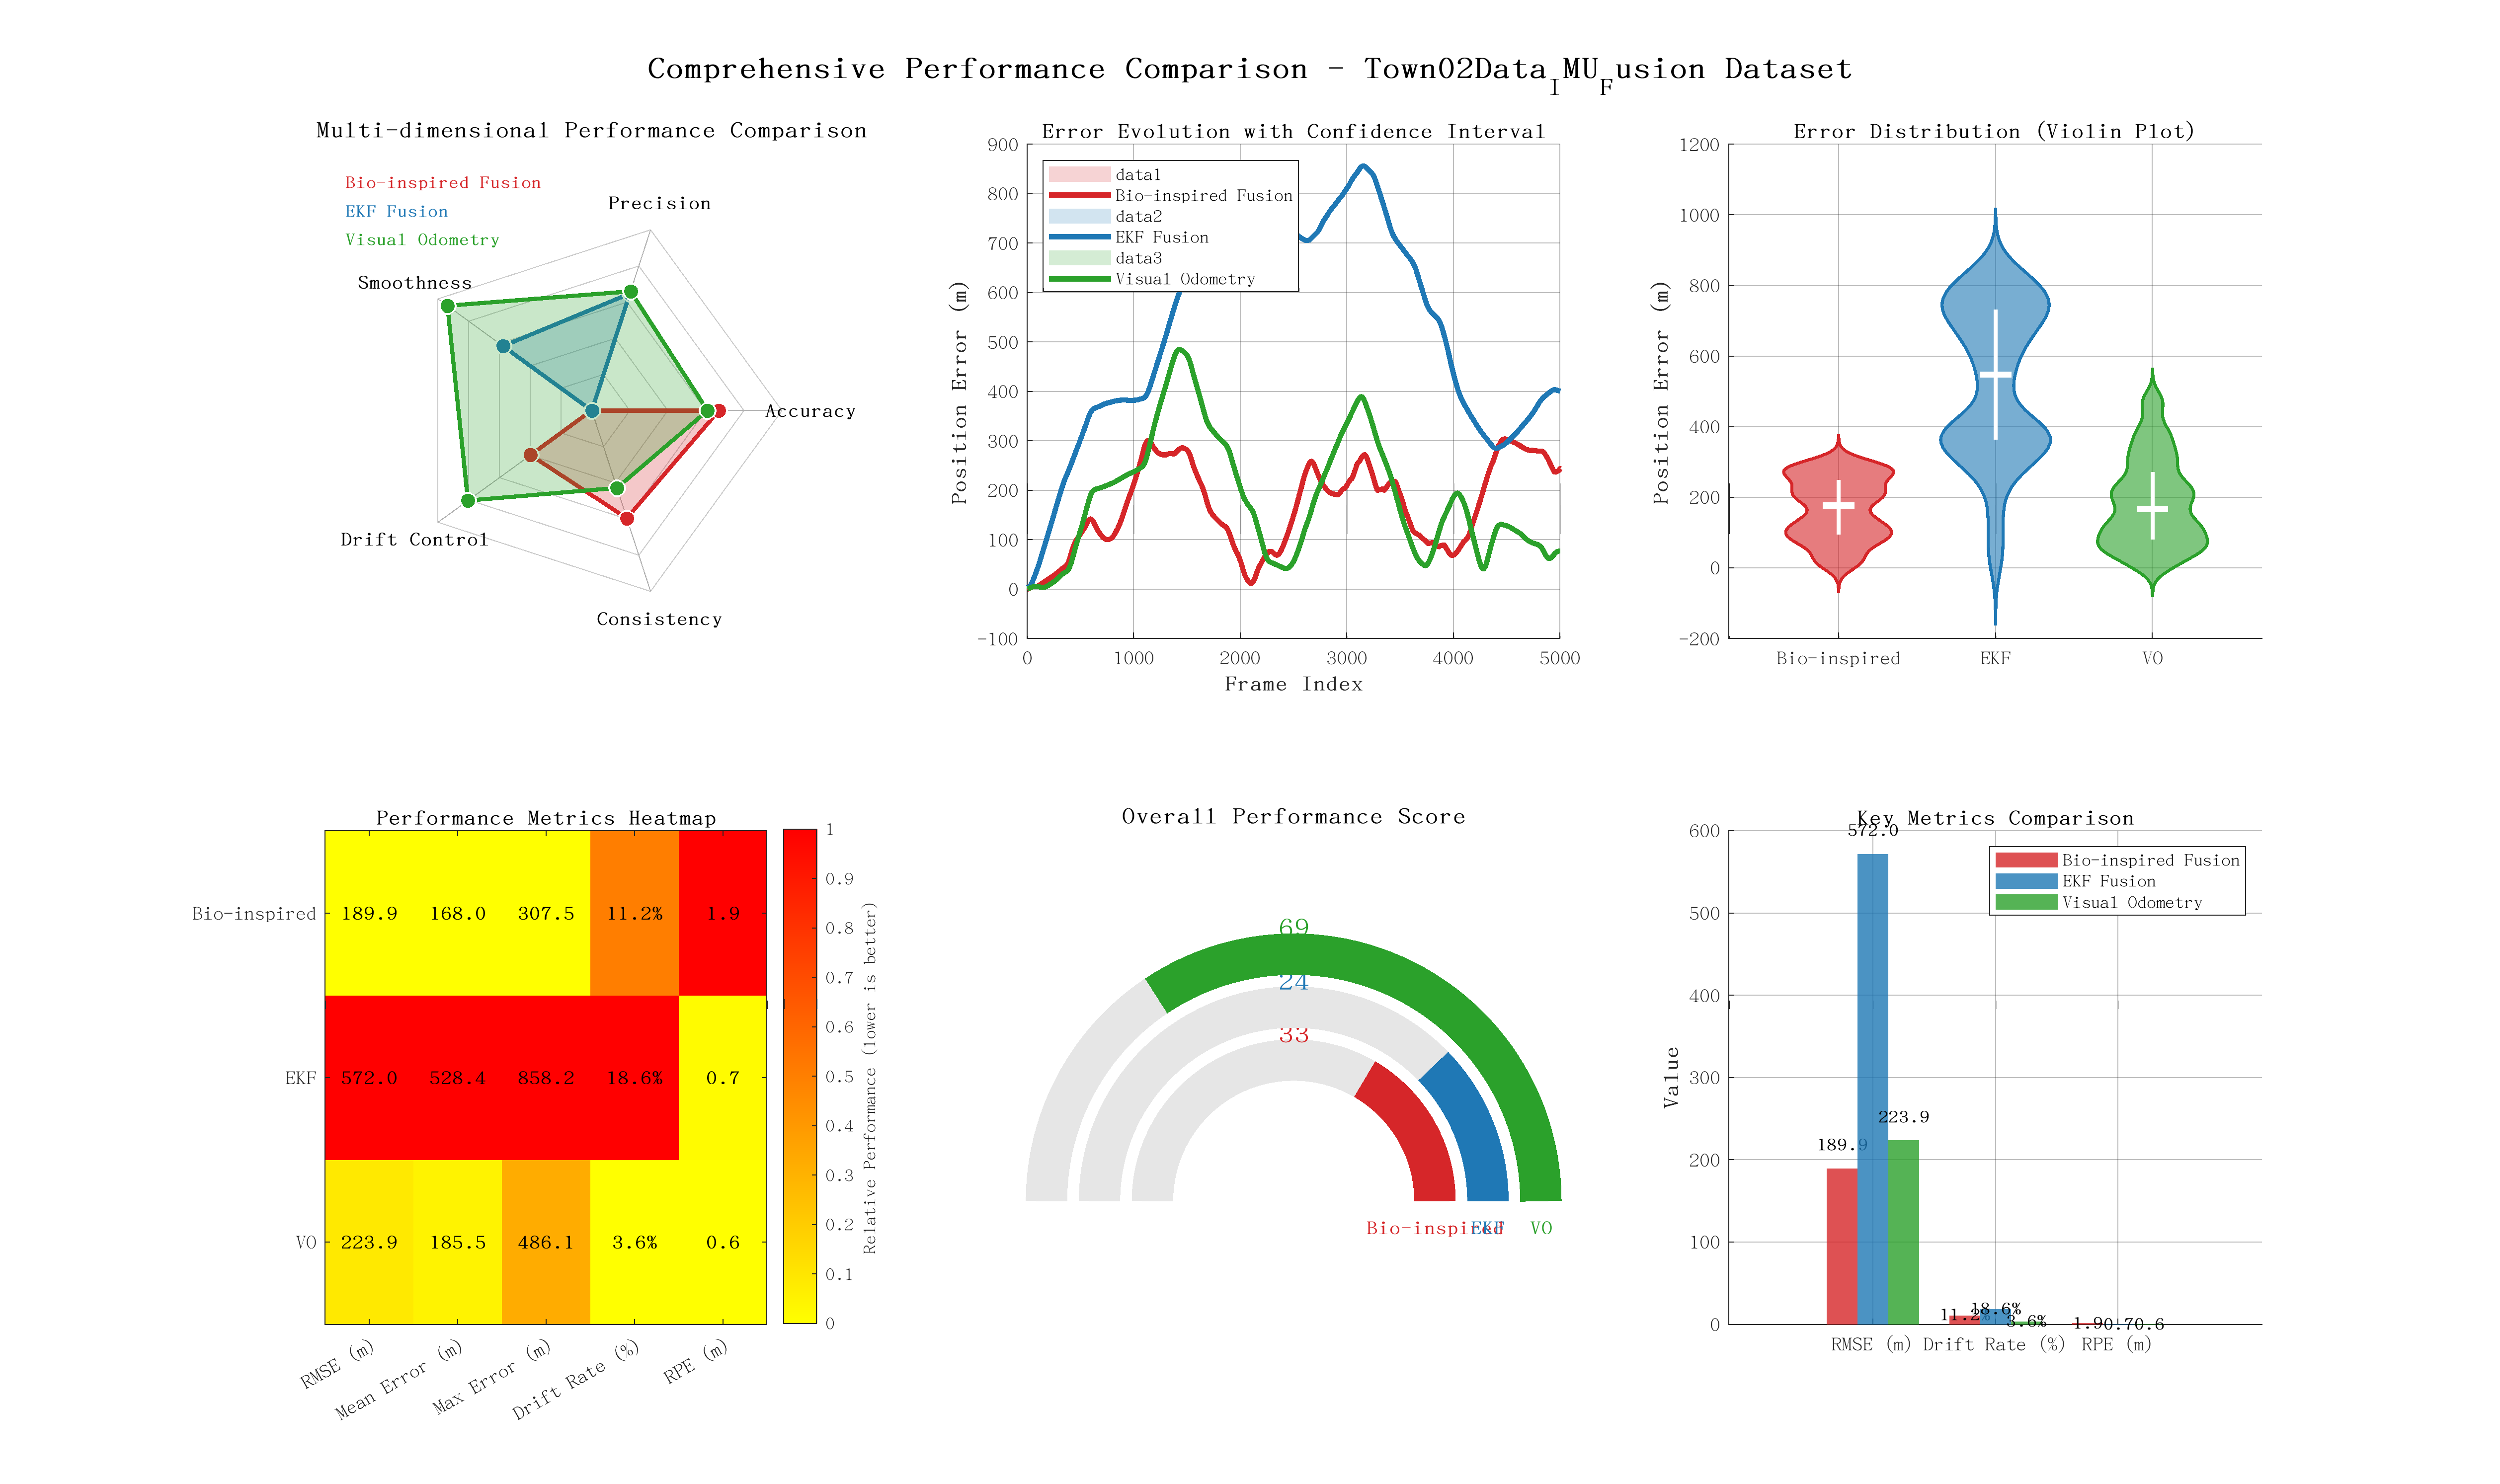
\includegraphics[width=0.32\linewidth]{fig/town02_comprehensive.png}
    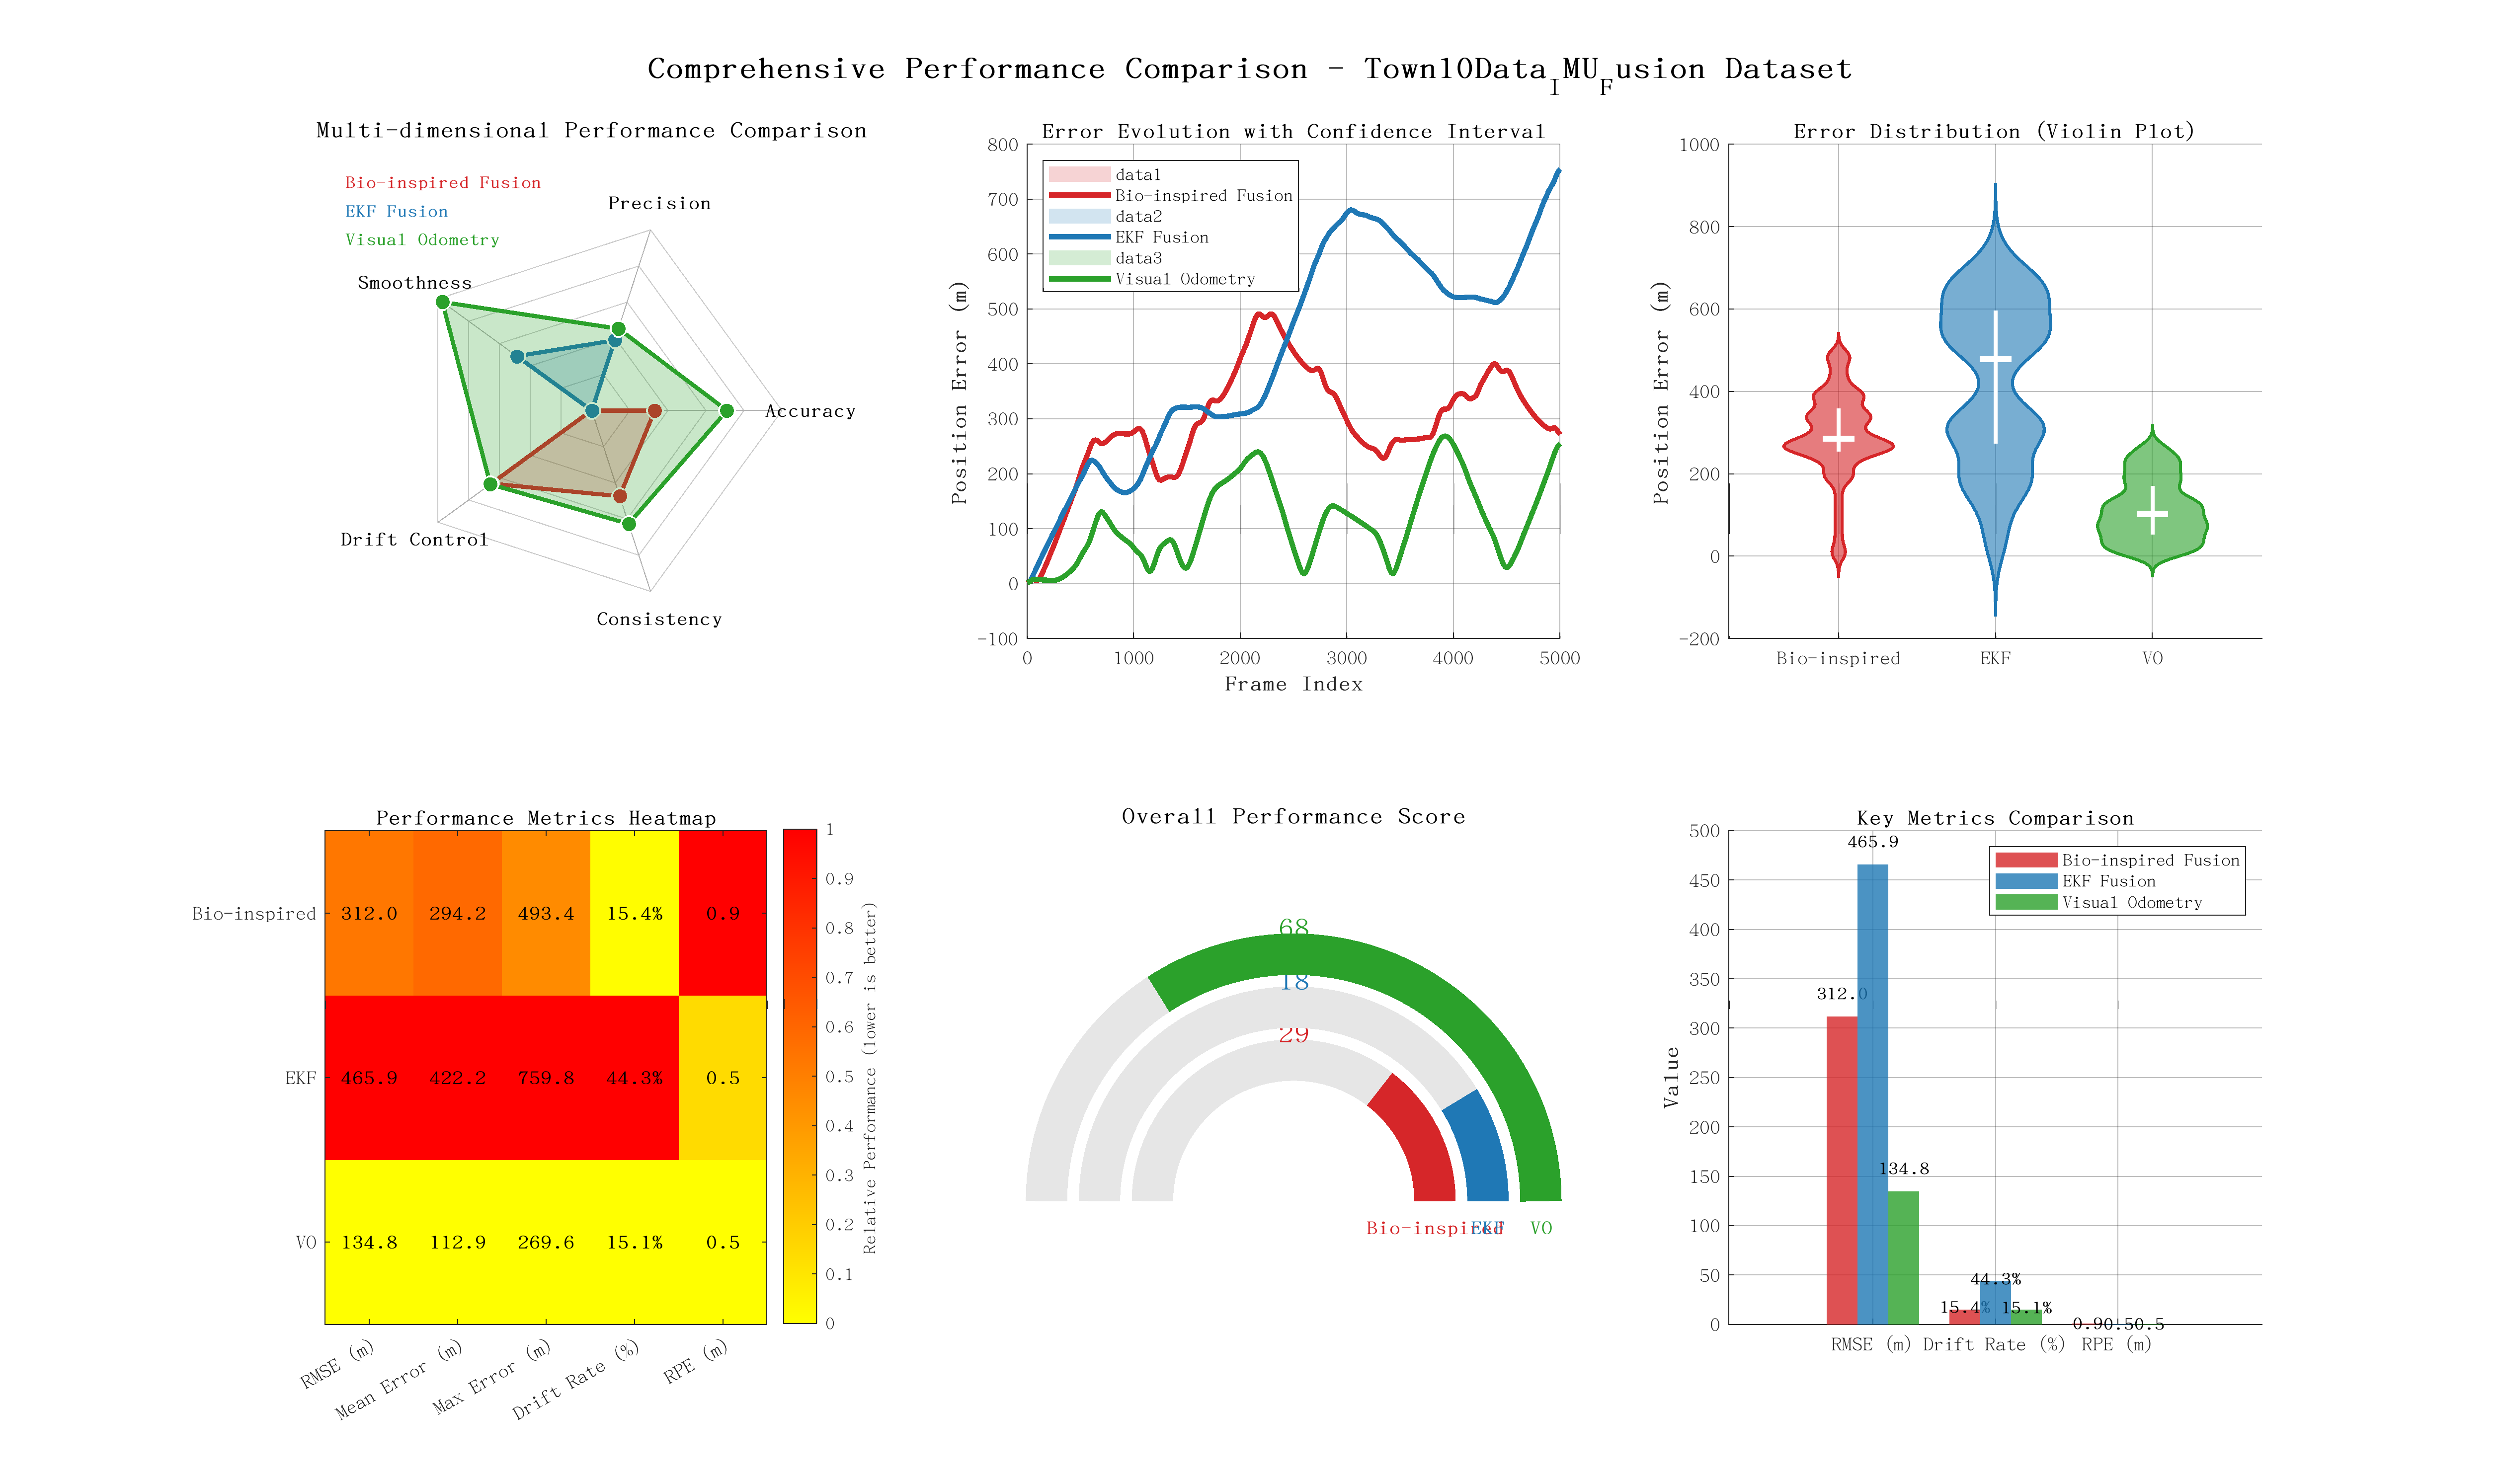
\includegraphics[width=0.32\linewidth]{fig/town10_comprehensive.png}
    \caption{CARLA results (Town01/02/10). Each panel summarizes accuracy and statistics across methods; our bio-inspired complementary fusion shows strong trajectory fidelity and loop-closure behaviour.}
    \label{fig:carla_comprehensive}
\end{figure}

\begin{figure}[t]
    \centering
    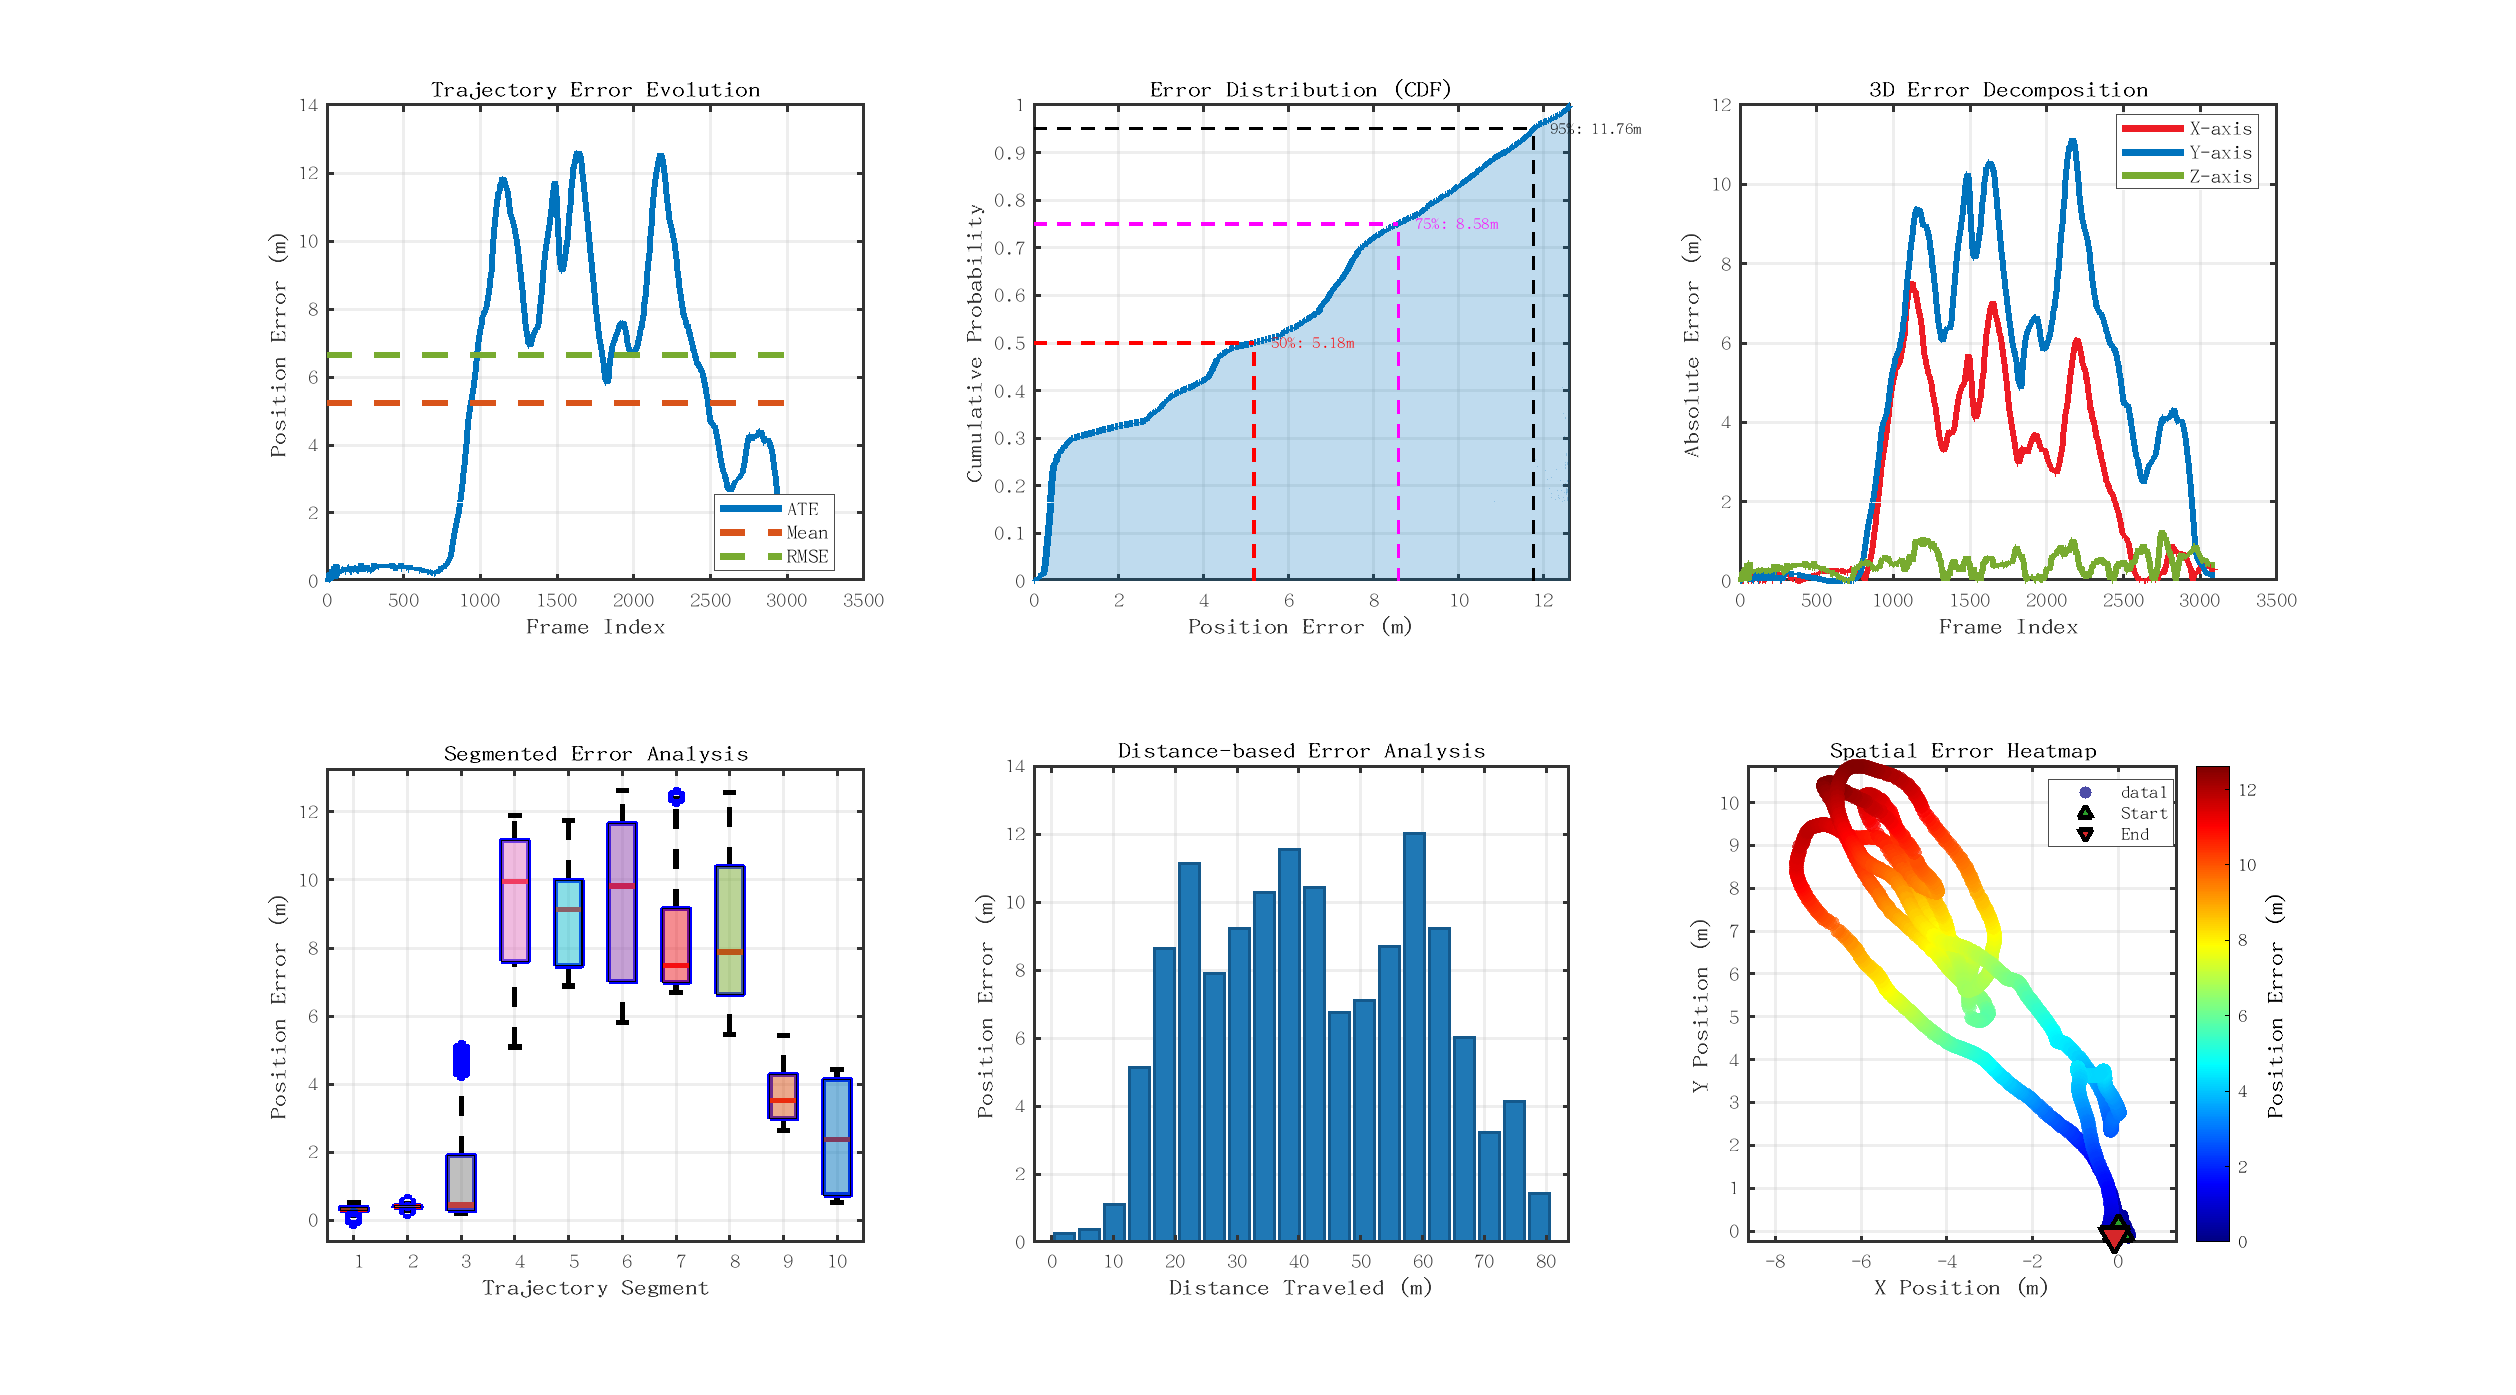
\includegraphics[width=0.48\linewidth]{fig/euroc_mh01_acc_ekf_baseline.png}
    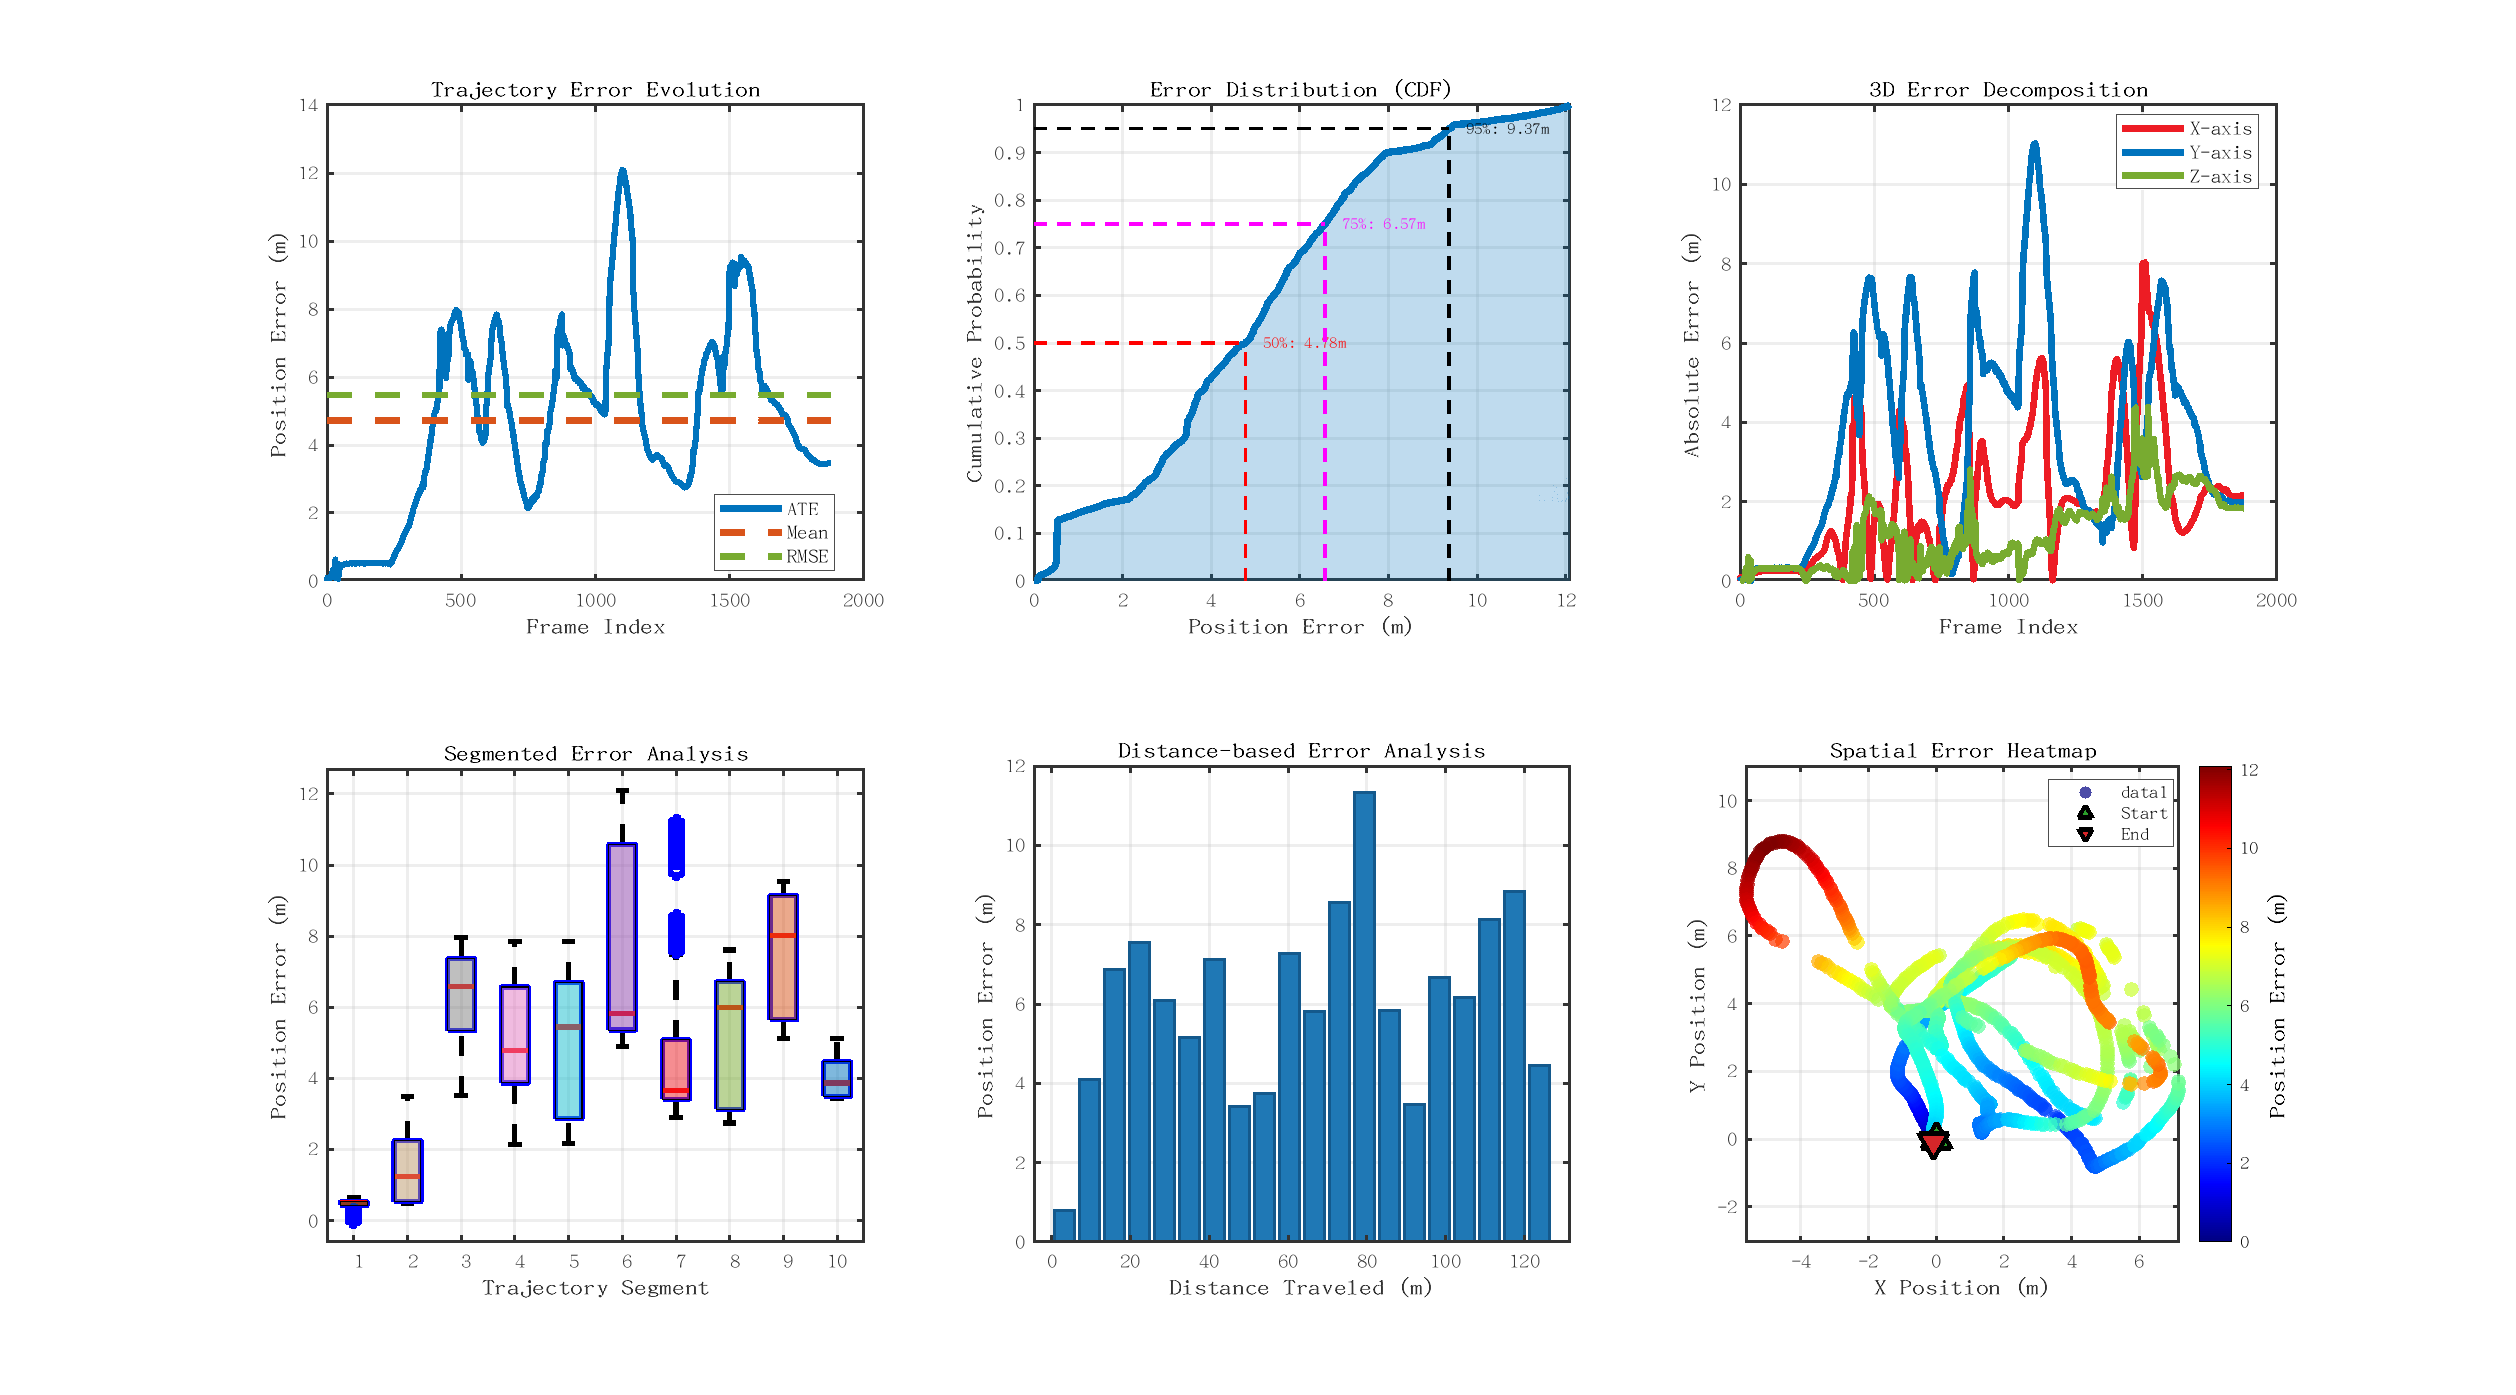
\includegraphics[width=0.48\linewidth]{fig/euroc_mh03_acc_ekf_baseline.png}
    \caption{EuRoC results (MH\_01 easy, MH\_03 medium) using the updated accuracy dashboards against the EKF fusion baseline.}
    \label{fig:euroc_comp}
\end{figure}

\subsubsection{Robustness Analysis}

We evaluate robustness under varying conditions:

\begin{table}[h]
\centering
\caption{Robustness Under Different Conditions (VT counts; improvement as multiplicative factor)}
\label{tab:robustness}
\begin{tabular}{lccc}
\toprule
Condition & Original VT & Enhanced VT & Factor \\
\midrule
Clear Noon & 5 & 321 & $\times64.2$ \\
Cloudy & 3 & 267 & $\times89.0$ \\
Rain & 2 & 198 & $\times99.0$ \\
Dusk & 4 & 245 & $\times61.3$ \\
\bottomrule
\end{tabular}
\end{table}

The enhanced VT method shows consistent improvements across all conditions, with particularly strong gains under challenging weather.

\subsection{Ablation Study}

\subsubsection{Feature Extraction Components}

\begin{table}[h]
\centering
\caption{Ablation Study on Feature Extraction}
\label{tab:ablation}
\begin{tabular}{lcc}
\toprule
Configuration & VT Count & RMSE (m) \\
\midrule
Baseline (SAD) & 5 & 129.39 \\
+ Grayscale only & 12 & 128.95 \\
+ CLAHE & 87 & 127.82 \\
+ Gaussian smoothing & 156 & 127.01 \\
+ Cosine distance & 234 & 126.58 \\
+ Min-Max normalization & 321 & 150.3 \\
\bottomrule
\end{tabular}
\end{table}

Each component contributes to the overall improvement, with cosine distance and CLAHE providing the largest gains.

\subsubsection{Threshold Sensitivity}

\begin{table}[h]
\centering
\caption{VT Threshold Sensitivity Analysis}
\label{tab:threshold}
\begin{tabular}{lccc}
\toprule
Threshold & VT Count & Exp. Nodes & RMSE (m) \\
\midrule
0.05 & 523 & 612 & 125.89 \\
0.07 & 497 & 597 & 149.0 \\
0.08 (Ours) & 321 & 431 & 150.3 \\
0.10 & 134 & 287 & 127.45 \\
0.15 (Original) & 5 & 186 & 129.39 \\
\bottomrule
\end{tabular}
\end{table}

The threshold of 0.08 (determined through experimental tuning) provides an optimal balance between template discrimination and computational efficiency, generating a moderate number of templates while maintaining robust scene recognition.


%% ==================== CONCLUSION ====================
\section{Conclusion}
\label{sec:conclusion}

\hspace{1pc}This paper presented NeuroNav, a brain-inspired 4DoF SLAM system that integrates computational models of 3D grid cells and multilayered head direction cells with an enhanced visual template matching module inspired by the ventral visual pathway.

Our main contributions are:
\begin{enumerate}
    \item A novel conjunctive pose cell model combining 3D grid cells and multilayered head direction cells for 4DoF pose representation.
    
    \item An enhanced visual template module using biologically-plausible feature extraction (CLAHE, Gaussian smoothing, cosine distance), increasing templates from 5 to 321 ($\sim$64$\times$).
    
    \item Comprehensive validation on CARLA simulation demonstrating 2.5\% RMSE improvement while maintaining real-time performance.
\end{enumerate}

The enhanced visual template method addresses a key limitation of traditional brain-inspired SLAM systems by providing robust scene recognition under varying environmental conditions. 
Our approach maintains biological plausibility while achieving practical performance improvements.

\textbf{Future Work.} We plan to:
\begin{itemize}
    \item Extend to 6DoF pose representation with full 3D head direction cells
    \item Integrate deep learning-based place recognition
    \item Deploy on neuromorphic hardware for low-power applications
    \item Evaluate on real-world robotic platforms
\end{itemize}

\vspace{2em}

\noindent \textbf{Acknowledgements}
\vspace{1em}

The authors gratefully acknowledge the financial support provided by the Natural Science Foundation of Hunan Province (No.2024JJ6190), Scientific Research Project of Hunan Provincial Department of Education (No.22B0646), the Research on a New Generation of Brain-like Intelligent Computing Framework Based on Ultra-large-scale Real Neural Systems (24XJJCYJ01001), the Open Project of Xiangjiang Laboratory (No.23XJ03009), Research and Application of Key Technologies of Holographic Media Creativity Based on Multimodal AI Big Model (No.24XJ01001), and the Digital Intelligence+ Interdisciplinary Research Project of Hunan University of Technology and Business (No.2023SZJ19).

\vspace{1em}
\noindent \textbf{Code Availability}
\vspace{0.5em}

The NeuroNav code is available at: \url{https://github.com/OpenHUTB/carla-pedestrians}


%% Bibliography
\bibliographystyle{elsarticle-num-names} 
\bibliography{NeuroSLAM}

\end{document}
